% !TEX root = ../rawlik-phd-thesis.tex
\chapter{Coil design} % Chapter title
\label{ch:coil_design}

\section{Introduction}
\marginpar{This chapter is largely adapted from the author's publication CITE WHEN AVAILABLE}
\note{Correct the langague and style to be consistent with the rest of the work. In particular, don't use so much \emph{we}.}
How to design a coil, or more generally, an arrangement of coils, producing a desired magnetic field? In its simplest form this is a textbook problem (e.g. ex. 6.55 and 6.62 in~\cite{Purcell}). Yet, in a general setting it is surprisingly hard and the solutions, how the wires making up the coils should be laid, complicated. The most widespread application of high-performance coils is Magnetic Resonance Imaging (MRI), where gradient coils give the possibility to produce spatial images. Already in the 1980's elaborate methods of MRI coil design have been developed. They range from optimizing positions of discrete windings, where the use is made of symmetries specific to MRI, to analytical methods yielding surface current density, which is then discretized. A general overview can be found in~\cite{Turner1993}. Another field known for complex, precise coils is plasma confinement, in particular stellarators~\cite{Beidler1990}. There analytical solutions for the surface current density find their use, too.

% \note{Cite also this: \cite{Del-Pino-Lopez2015}, they use a genetic algorithm to optimize the coils.}

Here, we present a new method that may not be competitive in terms of precision, but is distinct in its simplicity, also when it comes to construction of its designs. It relies on an algebraic representation of the problem, where coil design is simplified to a simple linear least squares problem. In our method the coils are restricted to a user-defined mesh, making it easy to deal with spatial constraints.

We base our discussion on textbook linear algebra techniques, notably solving an over-determined system of linear equations, thoroughly discussed e.g.\ in~\cite{Anton}. The main physics problem, calculating the magnetic field of coils composed of straight wire segments, is briefly discussed here. More in-depth discussions can be found, for example, in~\cite{Griffith}. Furthermore, we publish an easily accesible software implementation of the problems we discuss, including examples~\cite{Coilsjlcode}.

% The method has originally been developed to design coils of the active magnetic field stabilization system of the neutron electric dipole moment (nEDM) experiment at the Paul Scherrer Institute in Villigen, Switzerland. This application, described in detail in~\cite{Afach2014}, which we discuss later in the paper, requires large (6--8 meters side length) coils. In the presented method the coil system is designed on a predefined grid. This makes the construction of complicated coils feasible, despite the size.

We begin with a description of our model for a restricted 2-dimensional case and generalize it to three dimensions. We then present how the model is used to design a coil, based on an example. Further we discuss possibilities of simplifying the solution. Another section is devoted to practical considerations, significant for the eventual construction. Finally, we analyze the design method in the particular case of the magnetic field stabilization system of the nEDM experiment at the Paul Scherrer Institute.
\note{Last sentence baaaad.}



\section{Coils as a linear space}
Consider all possible coils that can be constructed by laying a wire on a surface of a square. The possibilities are endless. Speaking more precisely, as the wires may be shifted by arbitrarily small distances, as they overlap and cross, the problem has inherently an infinite number of degrees of freedom. We present an algebraic representation that reduces the number of degrees of freedom to just a few.

We start with a straight, finite wire segment spanned between points $\bm{x}_1$ and $\bm{x}_2$ (represented by vectors in an arbitrary coordinate system) and carrying current $I$, as depicted in Fig.\,\ref{fig:biot-savart}. To calculate the magnetic field it produces in the point $\bm{p}$, we use the Biot--Savart law. We consider the vector normal to the wire through the point $\bm{p}$:
\begin{equation}
  \bm{\rho} = (\bm{x}_1 - \bm{p}) - \left( \left( \bm{x}_1 - \bm{p} \right) \cdot \bm{n} \right)\bm{n} \ ,
\end{equation}
where $\bm{n}$ is a unit vector in the direction $\bm{x}_2 -\bm{x}_1$. The magnitude of the magnetic field in point $\bm{p}$ is then~\cite{Griffith}:
\begin{equation}
  \label{eq:biot_savart}
  B = \frac{\mu_0 I}{4 \pi \rho} \, \left| \sin \alpha_2 + s\, \sin \alpha_1 \right| \ ,
\end{equation}
where the angles $\alpha_i$ are not directed:
\begin{equation}
  \alpha_i = \frac{ \left\lVert \left( \bm{x}_i - \bm{p} \right) \times \bm{\rho} \right\rVert }{ (x_i  - p) \rho } \ ,
\end{equation}
and $s$ is $+1$ if $\bm{\rho}$ points onto the wire segment (between points $\bm{x}_1$ and $\bm{x}_2$) and $-1$ otherwise:
\begin{equation}
  s = \mathrm{sgn}\left( \tfrac{1}{2} \left\lVert \bm{x}_2 - \bm{x}_1 \right\rVert -
  \left\lVert \bm{p} + \bm{\rho} - \tfrac{1}{2} \left( \bm{x}_1 + \bm{x}_2 \right) \right\rVert \right)
\end{equation}
The direction of the field is given by the right-hand principle:
\begin{equation}
  \mathbf{B} = \frac{B}{\rho} \bm{\rho} \times \bm{n}
\end{equation}
This formulation is independent of the coordinate system (coordinate-system dependent solutions can be found e.g.\ in~\cite{Grivich2000}).

% (x1 .- p) .- ((x1 .- p) ⋅ n) * n

\begin{figure}
  \centering
  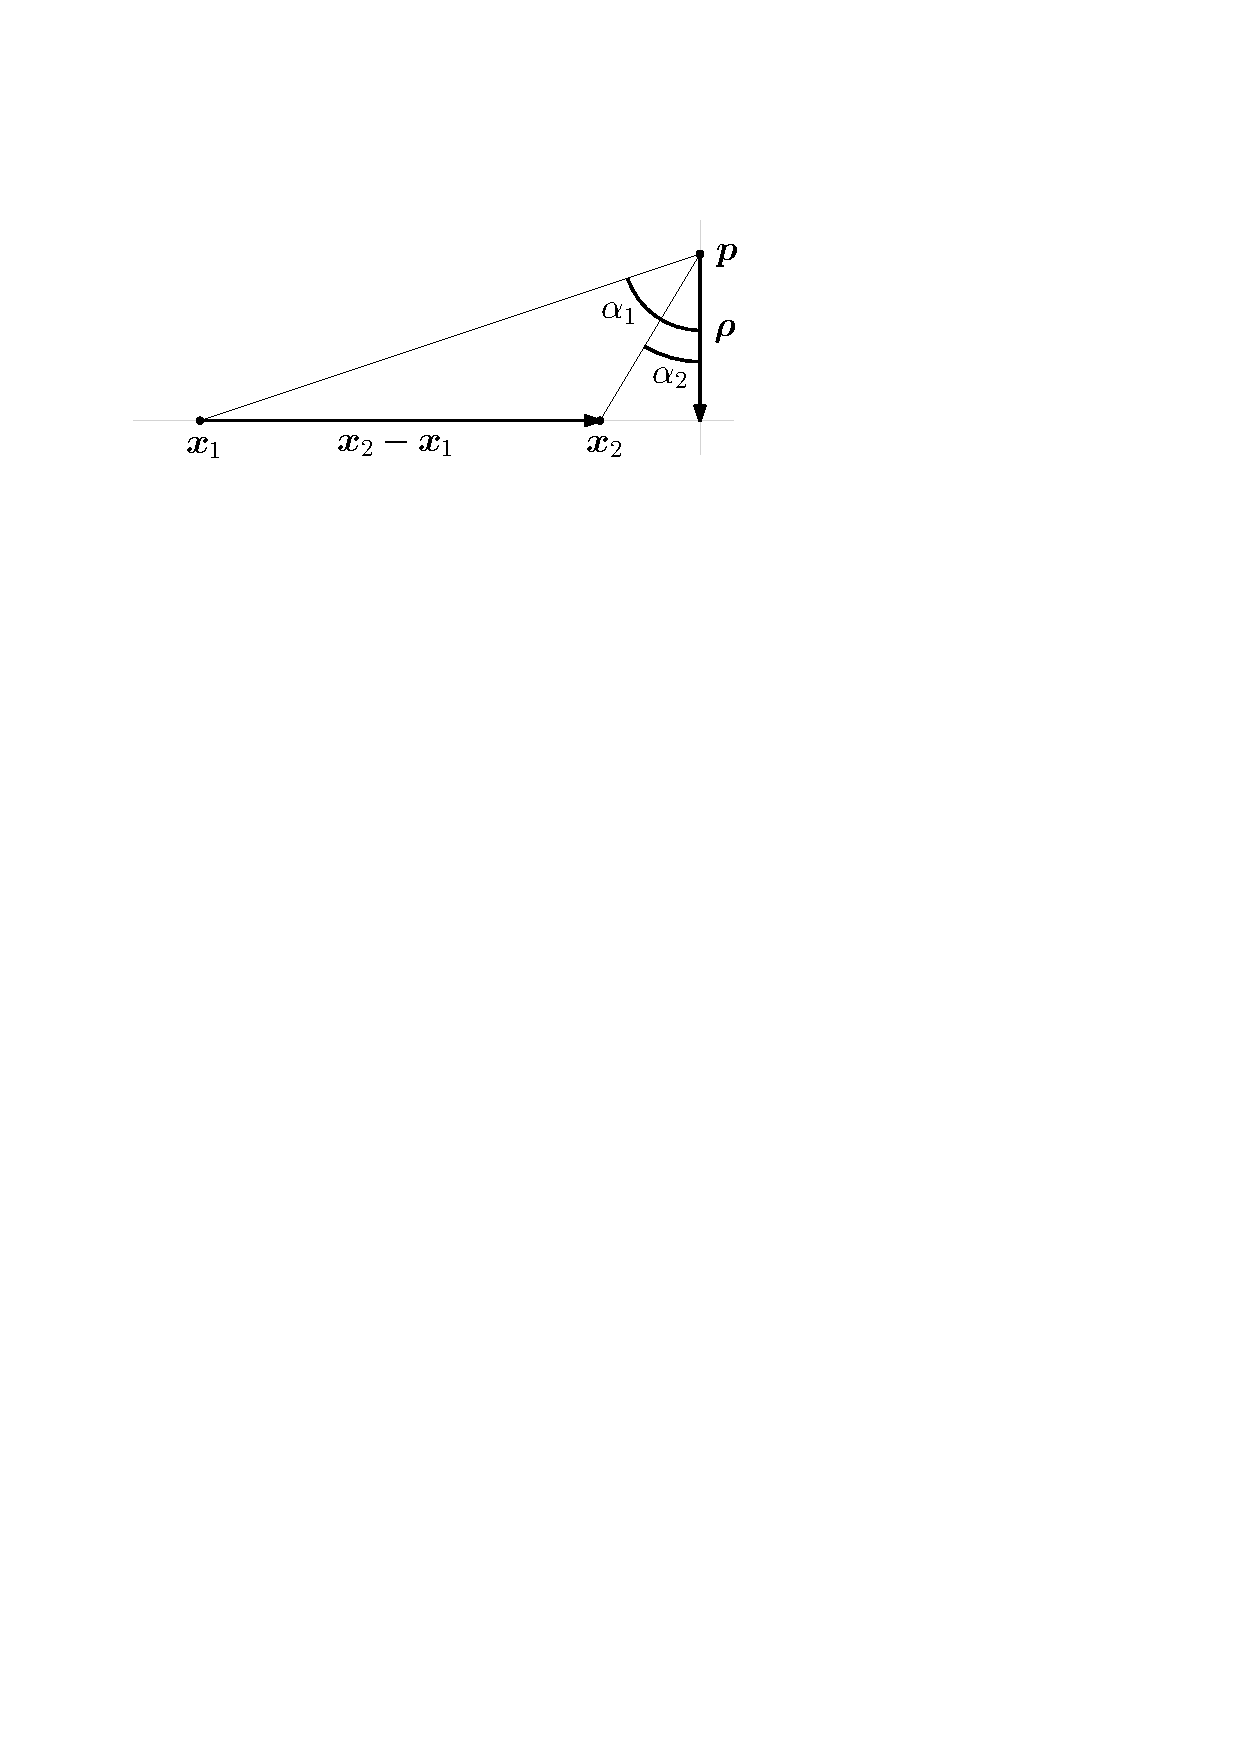
\includegraphics[width=0.6\linewidth]{gfx/coils/biot_savart.pdf}
  \caption{The setting for calculating the magnetic field produced in point $\bm{p}$ by a straight wire segment from $\bm{x}_1$ to $\bm{x}_2$.}
  \label{fig:biot-savart}
\end{figure}

Let us imagine four wire segments making up a square loop---a coil. It produces a certain magnetic field in the entire space $\mathbf{B}(\mathbf{x})$, given, following the superposition principle, by a sum of the fields produced by each segment of the coil.
By changing the current in the coil we alter only one parameter of the magnetic field---the magnitude, but not its shape. It can, therefore, be said that one coil spans a one-dimensional space of magnetic fields it can produce. Adding a second, different coil creates a system spanning a two-dimensional space of fields, as the magnetic field is additive. Going a step further, four square coils tiled to form a larger square form a four-dimensional space, as shown in Fig.\,\ref{fig:coils_tile_basis}. Any coil restricted to the $2 \times 2$ grid can be represented in the base of the four tile-coils.

The range of magnetic field reachable by coils restricted to a grid is a subset of all possible fields that can be created with coils constructed on the square's surface. The size of the subset is controlled by $N$, the number of tile-coils forming the grid.
% It is worthwhile to note that, in fact, a coil is equivalent to the field it produces . By constructing the grid we have thus restricted ourselves to a subset of \emph{coils} that are possible to construct on the square.
In this system a coil is fully described by a vector of $N$ currents, one in each of the tile-coils, denoted by $\mathbb{I}$. The problem of coil design is thereby simplified to finding a vector $\mathbb{I}$.
% The four coils form a complete linear basis of coils on the surface for any coils that have wires going only along the edges --- see Fig.\,\ref{fig:coils_tile_basis}. This is a very convenient subspace of all coils possible to build on a square. The possible to realise subspace may be enlarged by refining the division into tiles. But as a coil is equivalent to the field it produces, one can just as well say that they form a four--dimensional \emph{space of coils}.


\begin{figure}
  \centering
  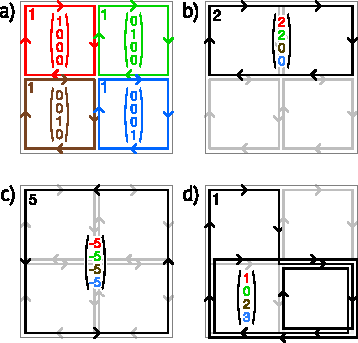
\includegraphics[width=0.6\linewidth]{gfx/coils/tile_basis.pdf}
  \caption{a) A basis of four tile coils on a flat square. Any coil which has its wires restricted to lie on the $2 \times 2$ grid can be represented as a linear combination of the four base tile coils. b, c, d) Three coils are presented together with their explicit coordinates in the basis.}
  \label{fig:coils_tile_basis}
\end{figure}

Generalisation onto a cube is simple, a cube being made up of six square faces. Interestingly, for the assembly in the three-dimensional space one degree of freedom is lost.  Figure~\ref{fig:coils_tile_kernel} illustrates, in the simplest case $N = 6$, a configuration in which finite currents in all six coils cancel and no magnetic field is produced. Such a combination of currents can be added to any solution with no effect on the produced field. Effectively, the space of the fields they can produce has dimension five (i.e.\ $N-1$). In other words, the mapping of $\mathbb{I}$ onto fields $\mathbf{B}(\mathbf{x})$ has in this case a one-dimensional kernel. This fact is of importance when it comes to numerically solving the system.

\begin{figure}
  \centering
  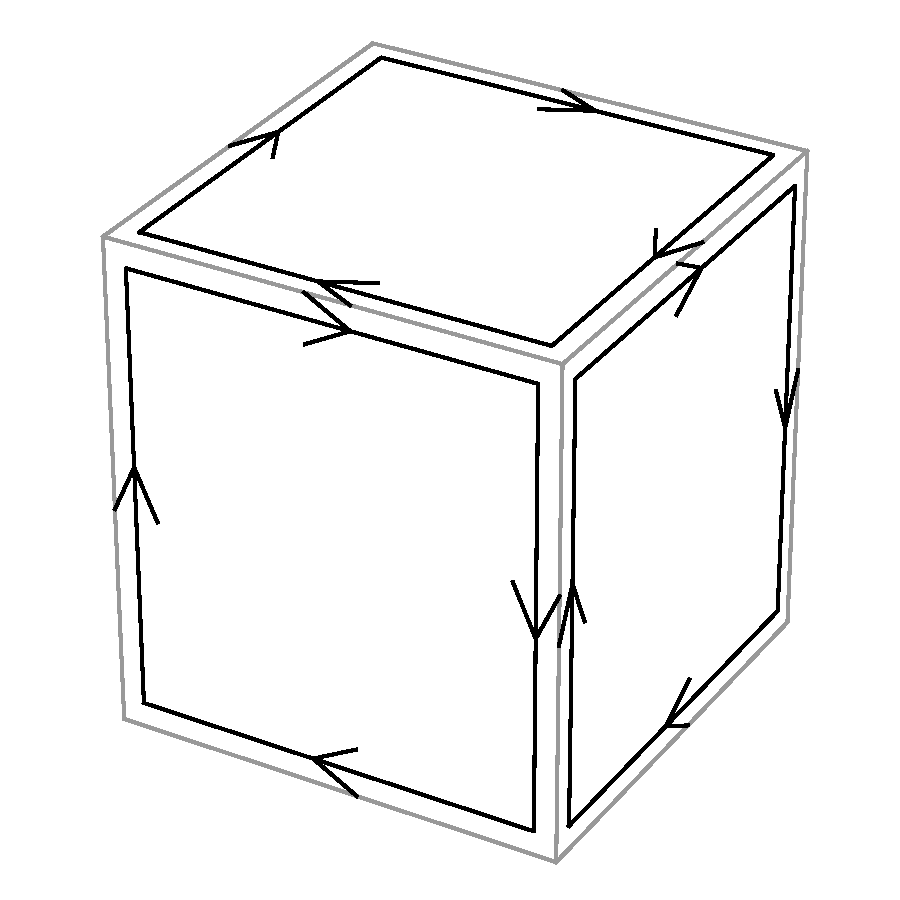
\includegraphics[width=0.5\linewidth]{gfx/coils/tile_kernel2.pdf}
  \caption{An arrangement of $N = 6$ tile coils on a cube which produces no magnetic field. The currents in the tiles are equal and flow in the directions as indicated. The currents on the invisible faces are analogous to the ones seen in front. For clarity, the coils are depicted slightly smaller; in the model the currents are identical with the edges of the cube.}
  \label{fig:coils_tile_kernel}
\end{figure}

This is the foundation of the method. We restrict our consideration to a grid on a cuboid, but in return we can fully describe all coils in the restricted space by a vector of $N$ numbers.



\section{Coil design}
In the problem of coil design one wants to create a coil, or an arrangement of coils, which best approximates a given field in a certain volume, which we will call \emph{the volume of interest}. Rather than considering the whole volume, we pick an ensemble of $m$ points of interest on its surface (the surface is sufficient because $\nabla \cdot \mathbf{B} = 0$). Hence, we look at the magnetic field $\mathbf{B}(\mathbf{x})$ only at these points and gather the values $\mathbf{B}(\mathbf{x}_i)$ for $i = 1 .. m$ into a vector of dimension $3m$ ($B_x$, $B_y$ and $B_z$ in each point), which we shall denote $\mathbb{B}$.

% Note, that magnetic field produced by a coil at a given point in space is proportional to the current in this coil. For a fixed direction in a fixed point in space it is a linear combination of currents of all coils in the system. Now, if we consider a vector of 3 spatial directions in $M$ points \ie, dimension $3M$. It can be obtained from an arbitrary coil $C$ by multiplying it by a $NNN \times 3M$ matrix $\mathbb{M}$. This matrix encodes the geometry of the system and may be pre-calculated.

As mentioned before, the magnetic field produced by a coil at any given point in space is proportional to the current in this coil. With many coils present it is a linear combination of the currents of all coils in the system. In absence of an external magnetic field the system of $N$ tiles and $m$ points of interest is thus described by a simple linear equation:
\begin{equation}
  \label{eq:matrix}
  \mathbb{B} = \mathbb{M} \, \mathbb{I}\ ,
\end{equation}
where $\mathbb{M} \in \mathbb{R}^{3 m} \times \mathbb{R}^{N}$ is a matrix of proportionality constants. For example, the element $\mathbb{M}_{(5, 2)}$ is the proportionality constant between the current in the second of $N$ coils and the magnetic field in the $y$ direction in the second of $m$ points of interest, $B_y(\mathbf{x}_2)$. The matrix $\mathbb{M}$ can be calculated analytically using the Biot-Savart law.

Equation~\ref{eq:matrix}, for $3m > N - 1$, is an over-determined system of linear equations, $\mathbb{I}$ being the vector of unknowns. We look for the optimal least-squares solution $\mathbb{I}_0$ to produce a $\mathbf{B}_0(\mathbf{x})$ in the volume of interest:
\begin{equation}
  \label{eq:requirement}
  % \mathbb{M} \, \mathbb{I} \stackrel{!}{=} \mathbb{B}_0
  \mathbb{I}_0 = \mathrm{arg}\,\min_{\mathbb{I}} \left( \mathbb{M} \mathbb{I} - \mathbb{B}_0 \right)^2 \ .
\end{equation}
The optimal solution can be calculated with the normal equation~\cite{Anton}:
\begin{equation}
  \mathbb{I}_0 = \left( \mathbb{M}^\mathrm{T} \mathbb{M} \right)^{-1} \mathbb{M}^\mathrm{T} \mathbb{B}_0 \ ,
\end{equation}
but the problem is typically solved numerically\footnote{\texttt{I0 = M \textbackslash{} B0} in MATLAB-like langagues.}. The majority of numerical software packages use the QR decomposition (a product of an orthogonal and upper-triangular matrix) of the matrix $\mathbb{M}$, which is more numerically stable when compared to the normal equation.

Depending on the properties of $\mathbb{M}$ the optimum may be multidimensional. In particular, as already mentioned, an arrangement of coils on a cube has a one-dimensional kernel, which will always cause the optimum to be at least one-dimensional. In these cases we will call $\mathbb{I}_0$ the unique least-norm solution, which minimizes the total current in the system. $\mathbb{I}_0$ is the vector of the optimal currents in the tile arrangement of coils for approximating $\mathbf{B}_0(\mathbf{x})$ in the volume of interest.

\begin{figure}
  \centering
  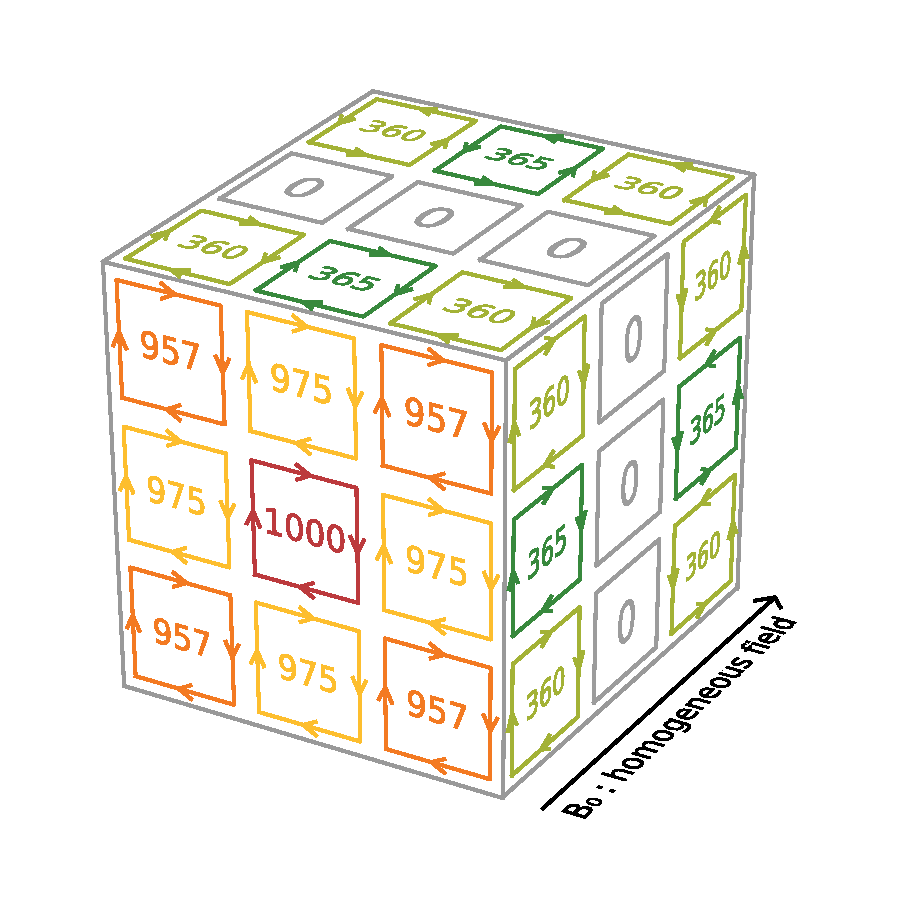
\includegraphics[width=0.6\linewidth]{gfx/coils/homogeneous_tiles_norm_1000.pdf}
  \caption{A solution of a tile system with $N = 6 \times (3 \times 3)$ tiles on a unit cube for a homogeneous field. The volume of interest is a cube with side length 0.75, centered inside the unit cube. Numbers indicate currents in the tile coils in arbitrary units. The currents are normalized so that the highest is 1000. For clarity, the coils are depicted slightly smaller; in the model their edges overlap. The currents on the three invisible faces are by symmetry analogous to the visible ones.}
  \label{fig:homogeneous_tiles}
\end{figure}

\begin{figure*}
  \centering
  \subfloat{
    \label{fig:homogeneous_performance_a}
    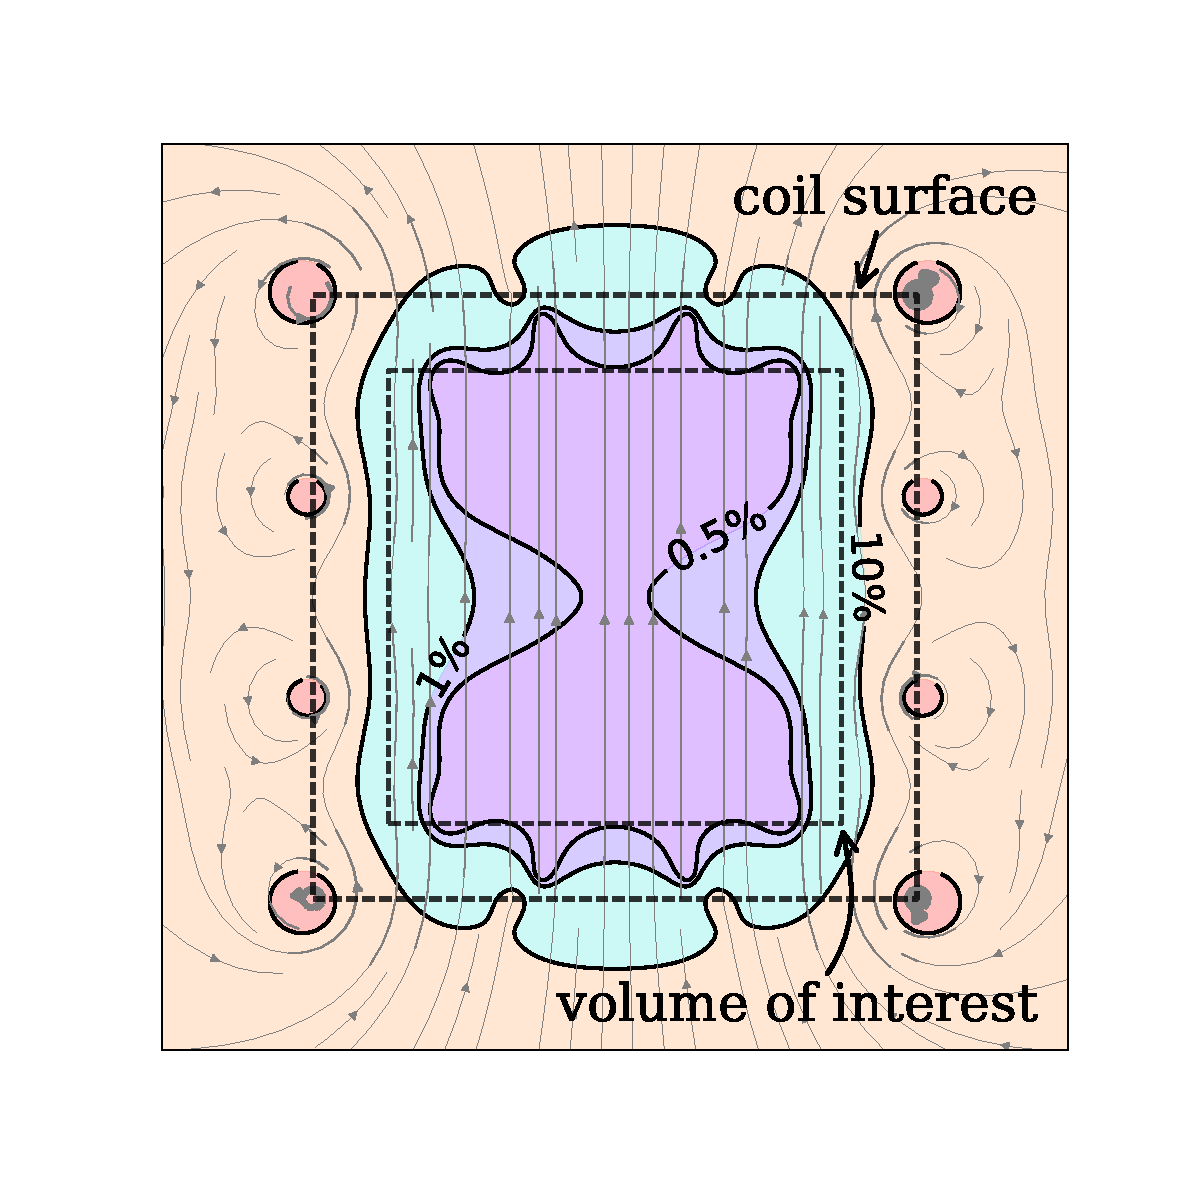
\includegraphics[width=.45\linewidth]{gfx/coils/homogeneous_performance.pdf}}
  \quad
  \subfloat{
    \label{fig:homogeneous_performance_b}
    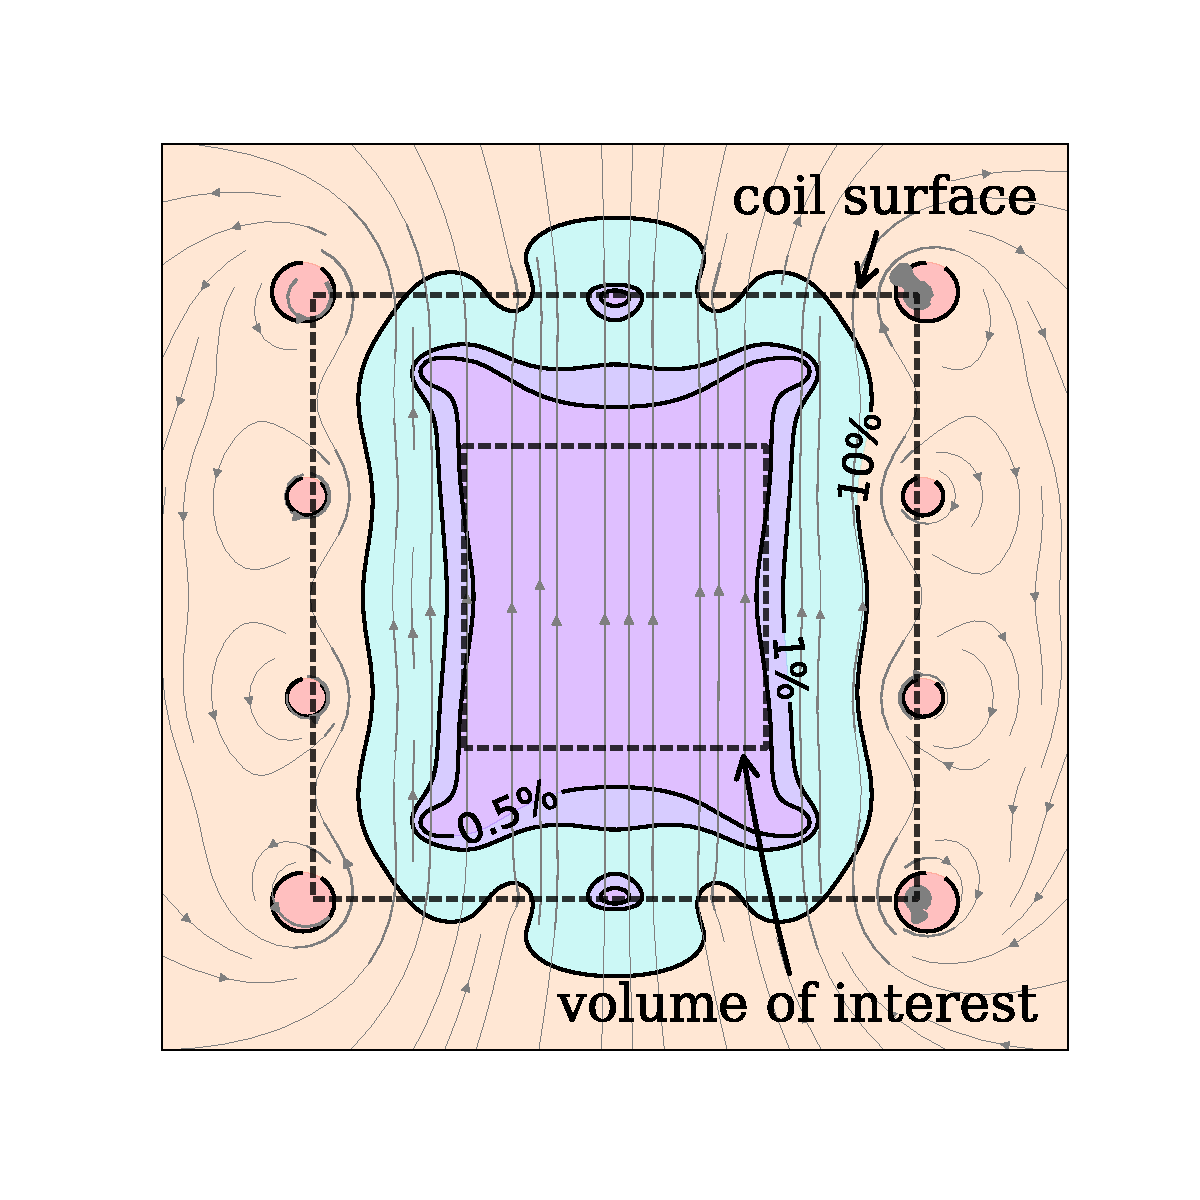
\includegraphics[width=.45\linewidth]{gfx/coils/homogeneous_performance_smaller_volume.pdf}}
  \caption{Magnetic field produced by a coil designed for a homogeneous field, with $N = 6 \times (3 \times 3)$ tiles on a unit cube. The field lines are depicted in grey. Contours show boundaries of 0.5, 1 and 10\% magnitude deviation from an ideal homogeneous field. Horizontal cross sections in the middle-height plane are shown. Two designs are presented. Left-hand side: the volume of interest is a cube with side length 0.75 (the individual tile coil currents are depicted in Fig.\,\ref{fig:homogeneous_tiles}), right-hand side: the size of volume of interest is reduced to 0.5.}
    \label{fig:homogeneous_performance}
\end{figure*}

Let us look at an example of a coil design on a unit cube with the number of tiles $N = 6 \times (3 \times 3)$ (see Fig.\,\ref{fig:homogeneous_tiles}). As the volume of interest we pick a cube, centered with the unit one, with side length 0.75 (with a regular mesh of $10 \times 10$ points on each face, a total of $m = 488$ points of interest). For the sake of simplicity we design a coil for a homogeneous field along an axis of the cube. The solution of Eq.\,\ref{eq:requirement}, $\mathbb{I}_0$, directly gives the currents in each tile, which are graphically depicted in Fig.\,\ref{fig:homogeneous_tiles}. Note that many currents almost cancel each other, in particular those along horizontal edges. The magnetic field produced by the solution is shown in Fig.\,\ref{fig:homogeneous_performance_a}, as a horizontal cut along the central plane. Contours show the relative deviation from the homogeneous field. Inside the volume of interest, depicted with a dashed line, the design goal of a homogeneous field, is reproduced with few per cent accuracy. The solution, and thus the contours too, depend on the choice of the volume of interest. In general, the further away the volume of interest is from the coils, the better the accuracy. If the side length of the volume of interest is decreased to 0.5, the accuracy improves to 1\%, as shown in Fig.\,\ref{fig:homogeneous_performance_b}. Note that the optimal solution, and thereby the shape of the precision contours, change. Naturally, the accuracy of the field reproduction can also be improved by increasing the number of tiles.

% The tile system may find an interesting practical application. Once independently controllable tiles have been build, it can be used to produce an arbitrary field. The precision is only limited by the number of tiles.


\section{Simplification of the tile system}
The tile system may find an interesting practical application. Once independently controllable tiles have been built, it can be used to produce an arbitrary field. However, building many independently driven coils is a high price to pay if one wants to produce only a simple field. Additionally, note that each edge is shared between two tiles, and the effective current is the sum of two. They may add either constructively or destructively. If the given solution is dominated by subtraction of large currents, a lot of power is unnecessarily dissipated in the system. It turns out that both problems can be solved by simplifying the tile solution.

\begin{figure*}
  \centering
  % \subfloat[A coil designed for a homogeneous $50\,\mathrm{\micro T}$ field along the x--axis. A net current along each edge is shown.]{
  %   \label{fig:coils_homogeneous_3d}
  %   \includegraphics[width=.45\linewidth]{coil_homogeneous}}
  % \quad
  % \subfloat[XY section in the middle --- achieved relative compensation of the homogeneous field.]{
  %   \label{fig:coils_homogeneous_section}
  %   \includegraphics[width=.45\linewidth]{coil_homogeneous_section}}
  % \\
  \subfloat{
    \label{fig:coils_dipole_3d_1}
    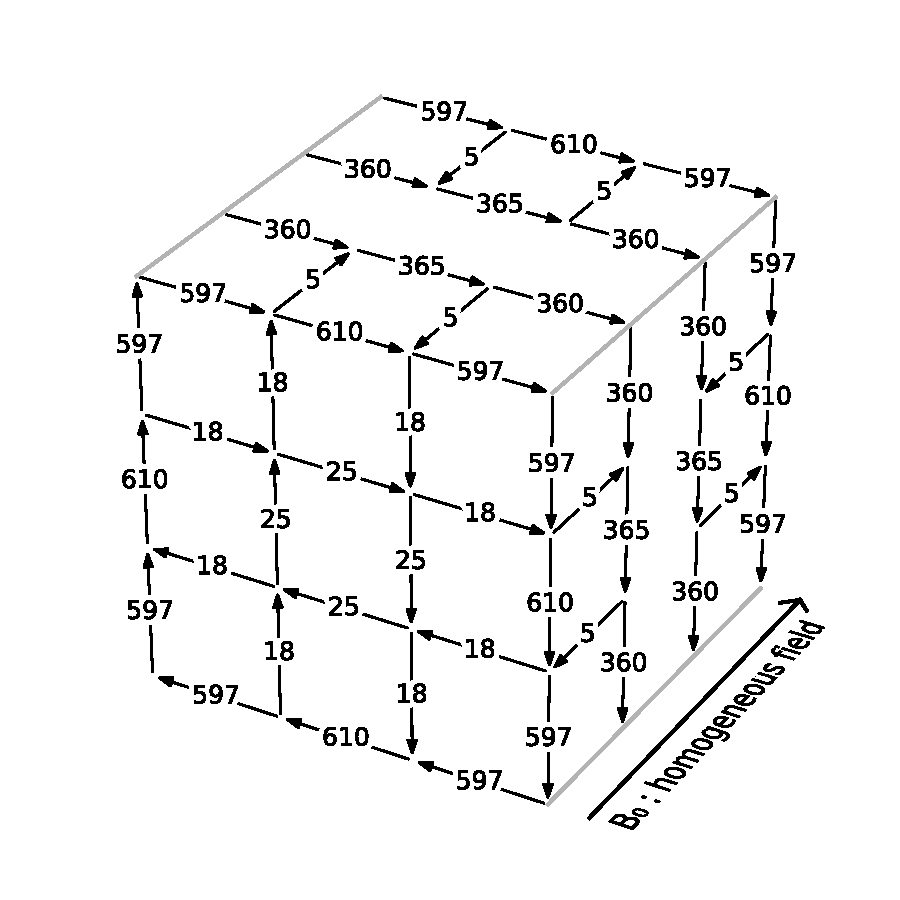
\includegraphics[width=.4\linewidth]{gfx/coils/algorithm_net_1.pdf}}
  \quad
  \subfloat{
    \label{fig:coils_dipole_section_0}
    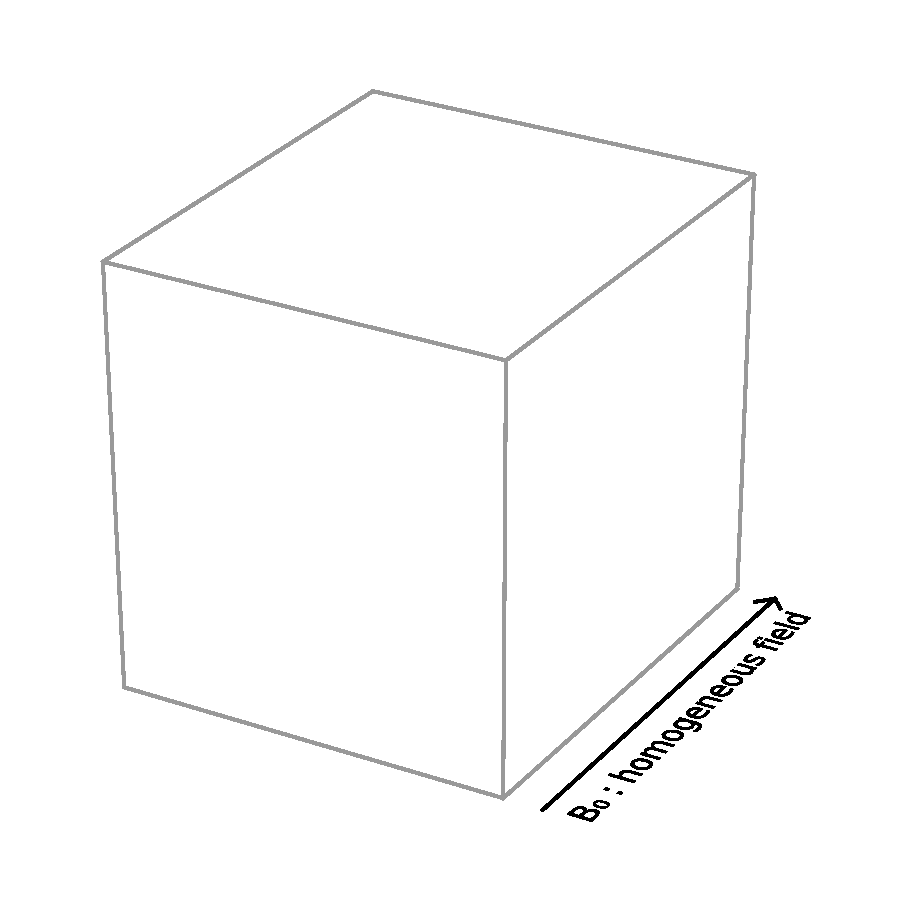
\includegraphics[width=.4\linewidth]{gfx/coils/algorithm_simplified_0.pdf}}
  \\
  \subfloat{
    \label{fig:coils_dipole_3d_3}
    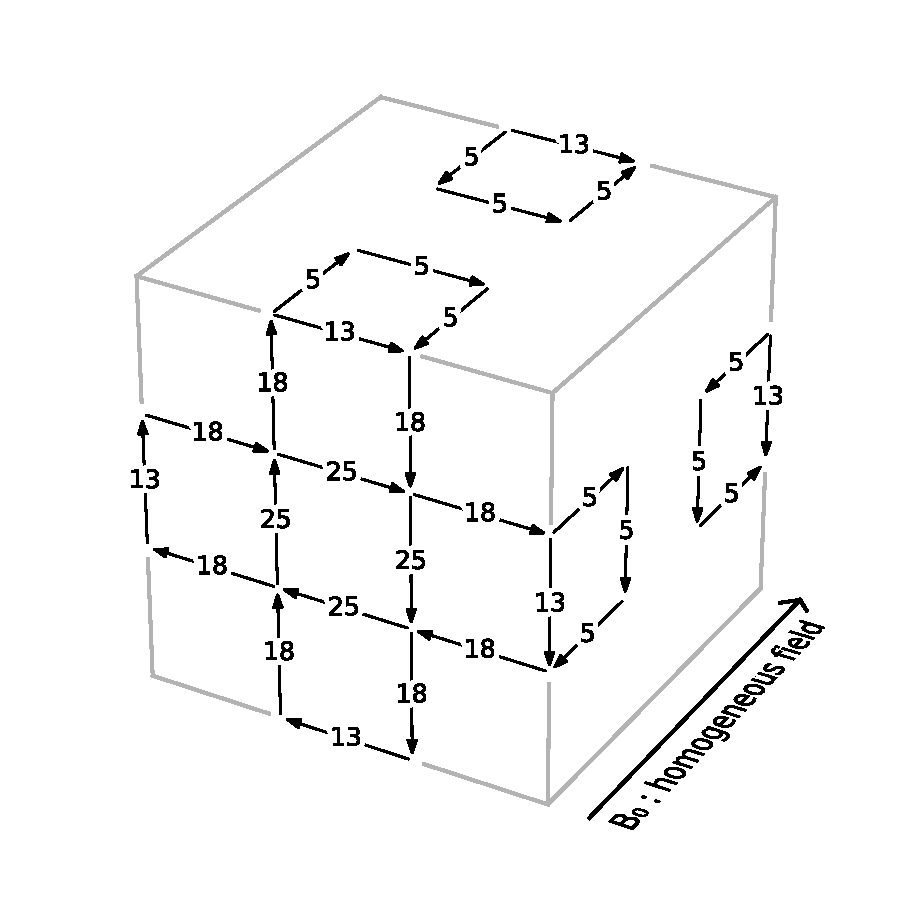
\includegraphics[width=.4\linewidth]{gfx/coils/algorithm_net_3.pdf}}
  \quad
  \subfloat{
    \label{fig:coils_dipole_section_2}
    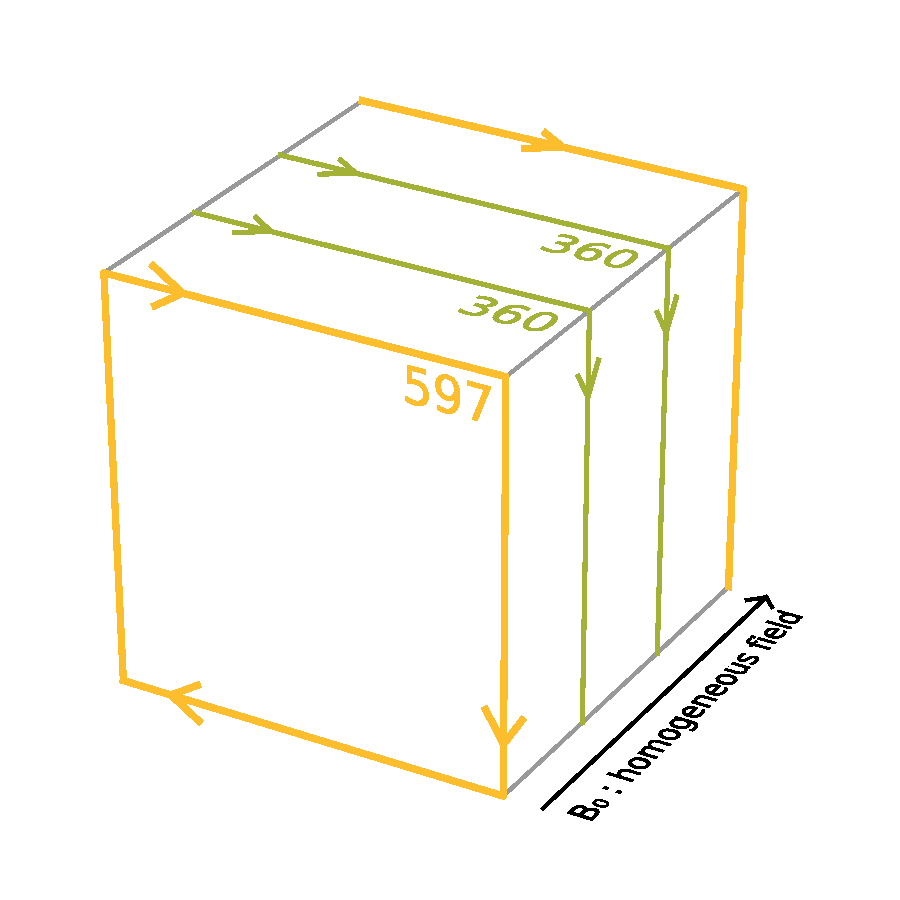
\includegraphics[width=.4\linewidth]{gfx/coils/algorithm_simplified_2.pdf}}
  \\
  \subfloat{
    \label{fig:coils_dipole_3d_5}
    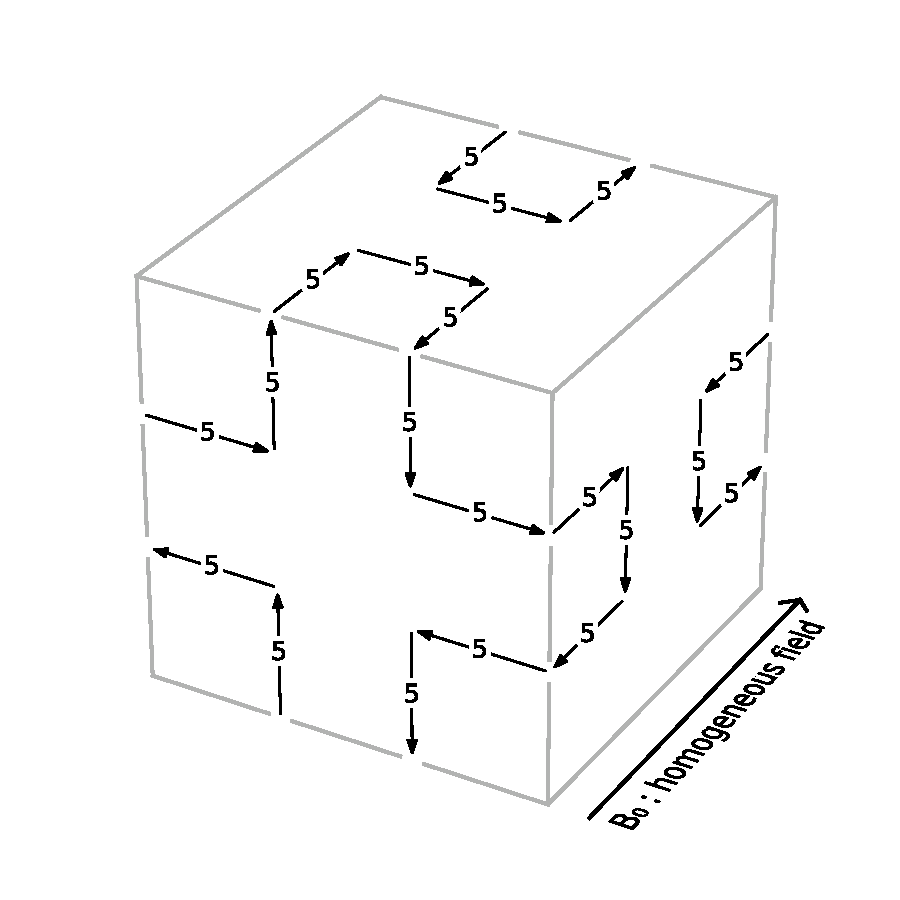
\includegraphics[width=.4\linewidth]{gfx/coils/algorithm_net_5.pdf}}
  \quad
  \subfloat{
    \label{fig:coils_dipole_section_4}
    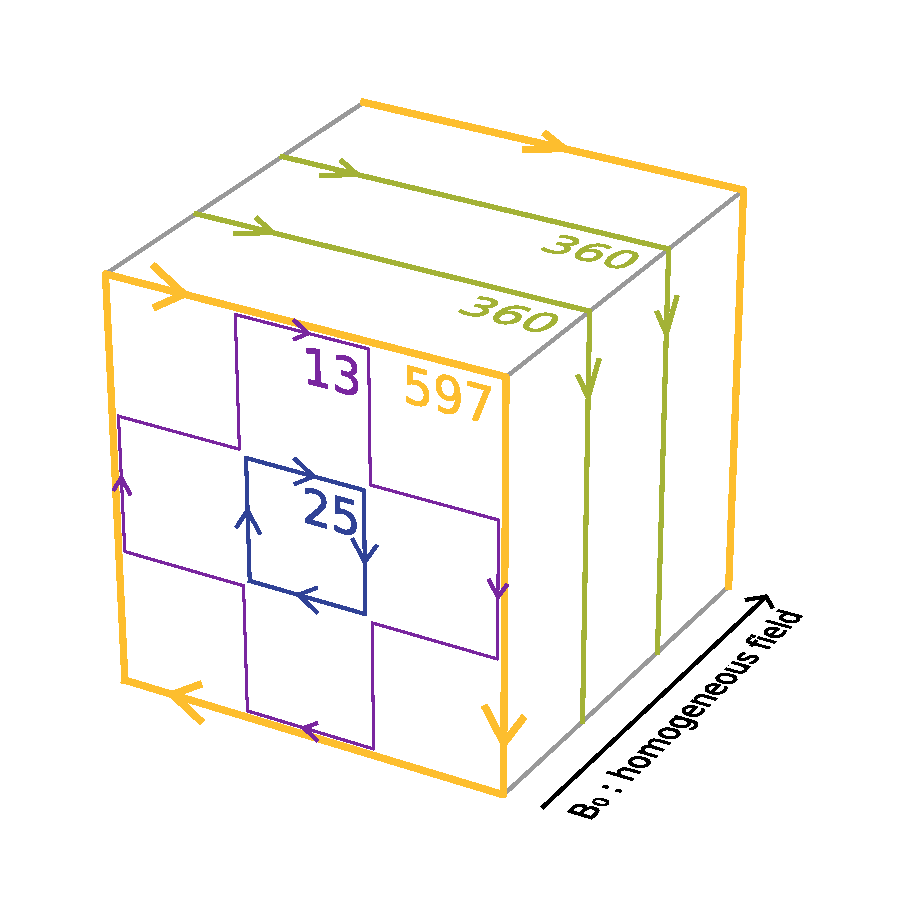
\includegraphics[width=.4\linewidth]{gfx/coils/algorithm_simplified_4.pdf}}
  \caption{Following the algorithm to simplify a coil. The left column shows the net of a current with the total current along edges of tiles. In each iteration the loop with the highest current is found and transferred onto the simplified solution, shown in the right column. We show iterations, from top: zeroth, fourth and eighth.}
  \label{fig:simplification_algorithm}
\end{figure*}

\begin{figure}
  \centering
  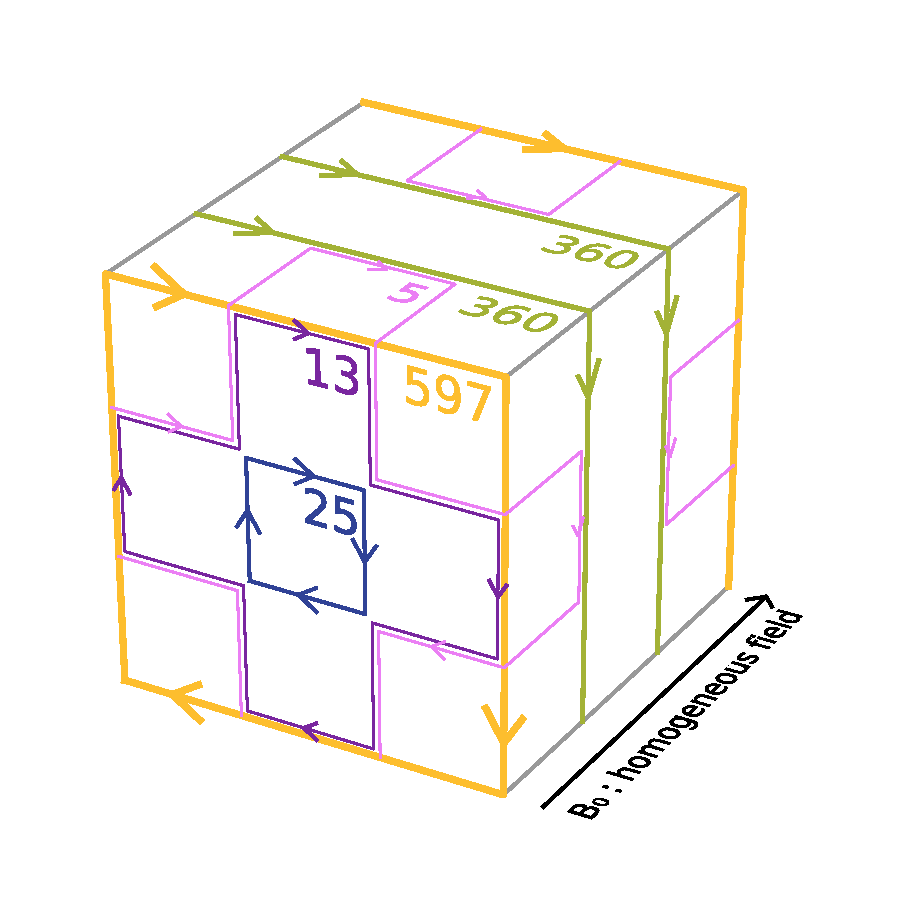
\includegraphics[width=0.6\linewidth]{gfx/coils/algorithm_simplified_5.pdf}
  \caption{The coil designed for a homogeneous field, with $N = 6 \times (3 \times 3)$ tiles (Fig.\,\ref{fig:homogeneous_tiles}), simplified by adding the currents along each edge and decomposing into current loops.}
  \label{fig:homogeneous_coils}
\end{figure}

One starts by adding the currents of the adjacent tiles and assigning the sum to each common edge. The result is a complicated net of currents (upper left corner of Fig.\,\ref{fig:simplification_algorithm}). Still, each node fulfills Kirchhoff's laws. The net can then be decomposed into simple current loops by following the algorithm: First find in the net the loop with the highest current. In the example it is either of the ``597" loops on the front and back faces. This loop will make the first one in the simplified solution (it can be seen in the middle of the right column in Fig.\,\ref{fig:simplification_algorithm}, together with the next three loops). Then subtract from the net the current of the first loop along its edges (the net that remains after subtracting the first four loops is depicted in the middle of the left column in Fig.\,\ref{fig:simplification_algorithm}). Finally, continue to find the loop with the highest current in the modified net, which will give the next loop and repeat until the current net is empty. The net remaining after eight loops are found is depicted in the bottom row of Fig.\,\ref{fig:simplification_algorithm}, next to the first eight loops. The final simplified solution is shown in Fig.\,\ref{fig:homogeneous_coils}. The currents in the simplified coil system are much smaller, the highest being 597 instead of 1000 and they always add constructively. Also the number of separate loops is decreased from 42 to 10. Still, the total current along each edge of a tile is exactly the same as in the tile configuration.

We conclude here our method of coil design. The simplified arrangement of coils is the optimal one, given the grid restriction, for approximating the magnetic field in the volume of interest. We continue to consider practical aspects, relevant for constructing the designs of our method.



\section{Practical considerations}
The primary practical advantage of our coil design method is that the coils are constrained to a predefined grid. This is contrary to other methods of coil design, where the position of the wires is the output of the procedure~\cite{Turner1993, Beidler1990}. This may prove useful in applications with spatial constraints. Typically, coils need to be incorporated into a setup in which other components penetrate the surface on which the wires are laid. In our method it is possible to simply define the grid so that no collisions occur. Although the simple examples presented before used regular grids, we have not used symmetries to solve the problem. When many coils are designed and built, for instance to produce homogeneous magnetic fields in each of the three dimensions, they can all share the same grid. The grid can, for example, be constructed out of cable channels into which the wires are laid.

A limitation associated with the finite size of the channels is the strength of the magnetic field that can be created, which, for given available power, is limited by the thickness of the wire. At the same the finite size of the cable channels can be neglected in the calculations only as long as it is small compared to the distance between the coils and the volume of interest. Using enameled wire, rather than standard, PVC-insulated cable, can reduce the overall thickness.

% Nooooo, make it more concrete!

% The size of the cable channels needs The finite size of the cable channels, especially for small systems.

% Using cable channels certainly would make it easy to build coil systems as large as many meters. When small systems are constructed, the effects associated with the finite size of the channels would become visible at some point. Another limitation associated with the finite size of the channels is the strength of the magnetic field that can be created, which, for given available power, is limited by the thickness of the wire. Using enameled wire, rather than standard, PVC-insulated cable, can reducte the thickness.

In our solution to produce the desired field one still needs a system of several coils, even in the simplified solution. The more complicated the goal field and the more tiles, the more different currents are needed across the individual loops, which quickly becomes impractical. There are several ways to tackle the problem.

The first way is to use only one current and adjust with the number of windings. In the example, when one decides for 60 as the maximum, then the current is $\mathrm{round}(597 / 60) = 10$. The 597, 360, 25, 13 and 5 would be created with 60, 36, 3, 1 and 1 windings respectively. A discretization error of $10 / 597 = 1.7\%$ is of the same order as the accuracy of the solution in representing the field (see Fig.\,\ref{fig:homogeneous_performance}). For more precise designs the numbers of windings get larger, which is troublesome to construct and causes the coils to have larger inductances.

A second way is to use a current divider. Connect the different loops in parallel, each with an appropriately chosen resistance in series. This way the ratios between the currents in each loop can be tuned precisely. However, a practical realization will most likely involve routing all loops out of the system where the current divider is installed. For more complicated coil systems with tens of different currents this may be impractical.

Yet another way is to split the loops into decades of currents. In the coil we use as an example the currents 597, 360, 13, 7, 5 (in arbitrary units) may be constructed from a set of wires with three relative currents of 100, 10 and 1, in the following way:
\begin{align*}
  597 & = 5 \times 100 + 9 \times 10 + 7 \times 1 \\
  360 & = 3 \times 100 + 6 \times 10 + 0 \times 1 \\
  13 & = 0 \times 100 + 1 \times 10 + 3 \times 1 \\
  7 & = 0 \times 100 + 0 \times 10 + 7 \times 1 \\
  5 & = 0 \times 100 + 0 \times 10 + 5 \times 1 \\
\end{align*}
In this way one can reach better than 1\% accuracy in reproducing the solution in practice with only 3 different currents to control, even for complicated designs. Those can be either separately controlled or split with a current divider.

We do not consider any of the above ways superior. It is up to the particular application which is the best suited one.



\section{Application to active magnetic field shielding}
Using the method presented here to design coils of an active compensation system offers improvements in two areas. Firstly, the size of the coils could be decreased, or the size of the experimental set-up increased, without loss of performance. Better homogeneity in a given volume can always be achieved by choosing a denser gird. Given the tight spatial constraints this was a crucial development for the design of the n2EDM's active compensation system.

\begin{table}
  \centering
  \begin{tabular}{c|ccc}
    n & $\mathbf{P}_n^x(\mathbf{r})$ & $P_n^y(\mathbf{r})$ & $P_n^y(\mathbf{r})$ \\ \hline
    1 & 1 & 0 & 0 \\
    2 & 0 & 1 & 0 \\
    3 & 0 & 0 & 1 \\ \hline
    4 & $x$ &  0  & $-z$ \\
    5 & $y$ & $x$ &   0  \\
    6 &  0  & $y$ & $-z$ \\
    7 & $z$ &  0  & $ x$ \\
    8 &  0  & $z$ & $-y$ \\
  \end{tabular}
  \caption{Carthesian harmonic polynomials.}
  \label{tab:coils_carthesian_harmonics}
\end{table}

Secondly, the method allows to construct a coil for any field. In particular, one may choose to construct coils that produce fields orthogonal to one another. 
% (as $\mathbb{R}^3 \rightarrow \mathbb{R}^3$ functions).
This makes a compensation system significantly easier to control~\cite{MRM:MRM1910010107} and avoids a potential problem of the high condition number due to very-high-order fields produced by pathological combinations of coils. One of the possible orthogonal decompositions of the field is the one into \emph{cartesian harmonic polynomials}~\cite{Franke2013}:
\begin{equation}
  \mathbf{B}(\mathbf{r}) = \sum_{n}\,H_n \mathbf{P}_n(\mathbf{r}) \ ,
\end{equation}
where $H_n$ are the expansion coefficients, and $\mathbf{P}_n(\mathbf{r}$ are the cartesian harmonic polynomials, the first eight of which are listed in Table~\ref{tab:coils_carthesian_harmonics}. Each term satisfies by itself the Maxwell's equations, so it is possible to construct a coil for each. The first three terms are homogeneous fields, the next five are the five independent linear gradients. Further ones correspond to higher-order gradients.

\begin{figure*}
  \centering
  \subfloat{
    \label{fig:coils_dipole_3d}
    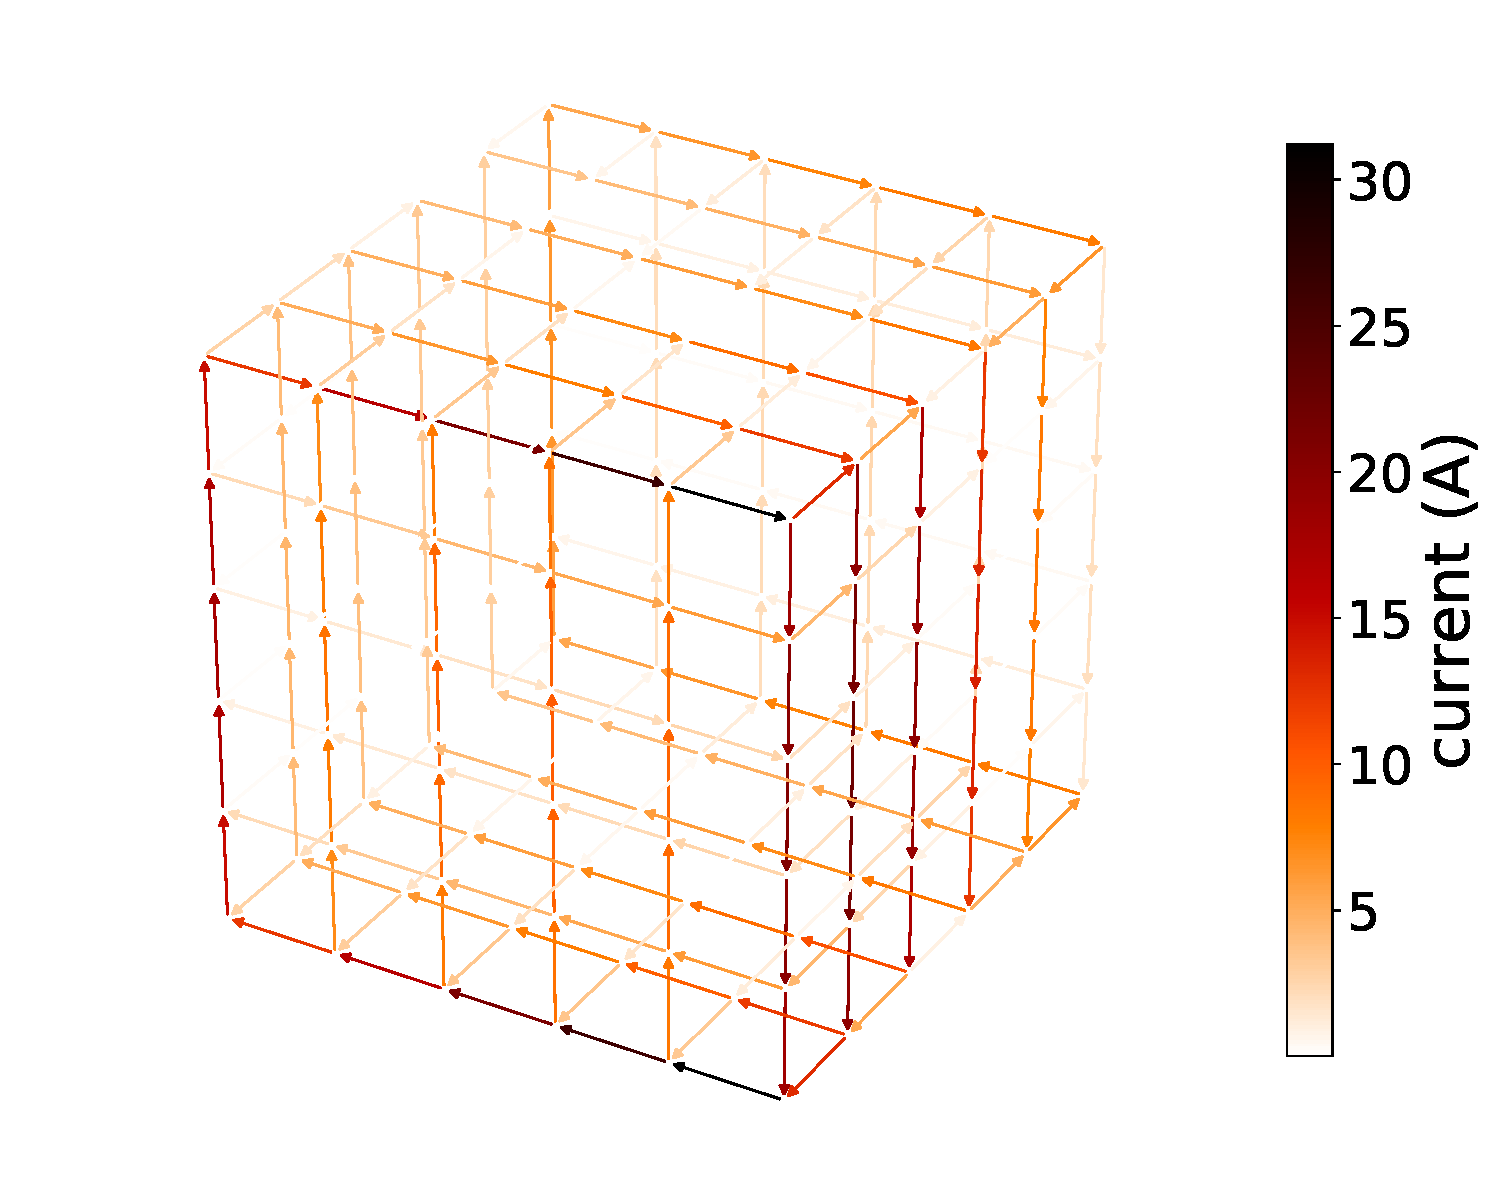
\includegraphics[width=.35\linewidth]{gfx/coils/coil_dipole.pdf}}
  \quad
  \subfloat{
    \label{fig:coils_dipole_section}
    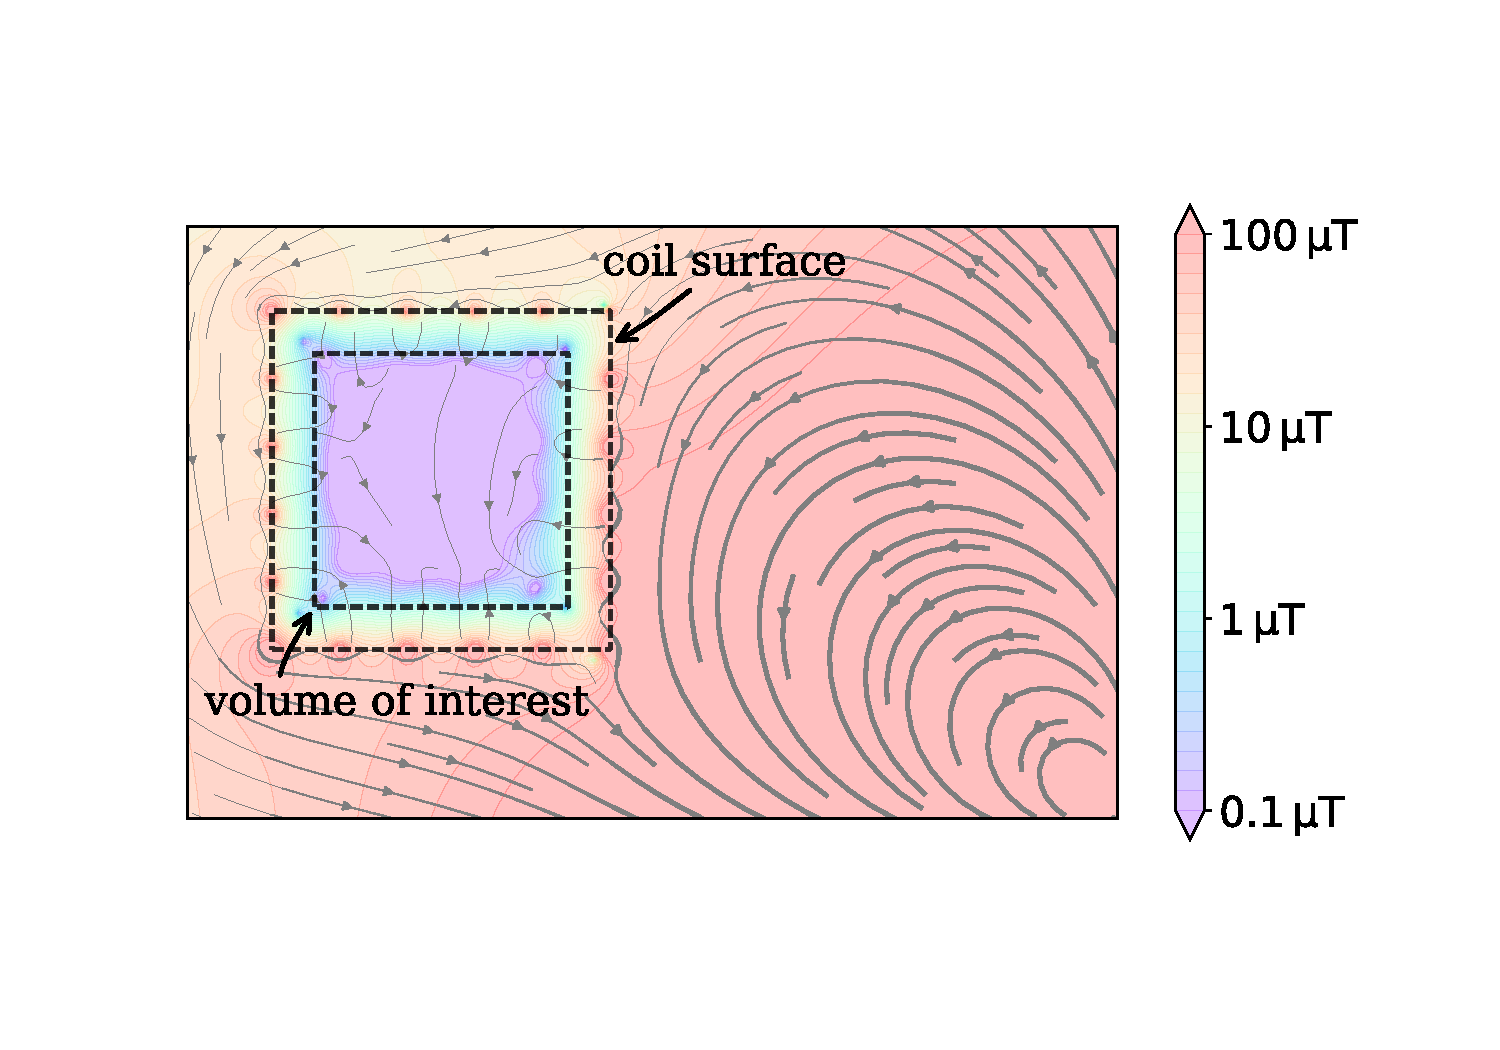
\includegraphics[width=.55\linewidth]{gfx/coils/coil_dipole_section_with_dipole.pdf}}
  \caption{A coil designed on a unit cube with $5 \times 5$ tiles per face to shield against a dipole disturbance. The dipole is located, relative to the center of the unit cube, two units to the right and one unit to the front. It is located in the middle height of the cube. The volume of interest has a side length of 0.75. On the left-hand side the total current along each edge of the dipole compensation coil is depicted. On the right-hand side the magnetic field is shown. The magnetic field lines are shown in grey, the volume of interest and the coil surface with dashed lines. The colors depict the magnitude of the magnetic field (capped at 0.1 and 100\,µT). A horizontal cross section in the middle height is shown. The dipole source is located in the lower right corner of the plot and points parallel to the plane of the plot. The magnitude of the field in the volume of interest is reduced from tens of microteslas down to below one.}
  \label{fig:showcase}
\end{figure*}

Additionally, one can consider constructing dedicated coils to counteract a particular known disturbance. In Fig.\,\ref{fig:showcase}, a showcase design with $N = 6 \times (5 \times 5) = 150$ tiles for compensating a nearby dipole source is presented.

Last, but not least, the method's unique property of designing on a predefined grid makes a large-scale construction particularly feasible. It makes it easy to be incorporated into the existing structures, by defining the grid in a conflict-free way first.



\section{Conclusion}
Coil design is a complicated and very technical problem, especially when high accuracy is required. We presented a method that is simple in terms of both underlying math and computational effort. We believe that the design method can find its niche in practical applications, where spatial constraints play a significant role and a percent level in accuracy of the produced field is acceptable.

The method has particular advantages when used to design coils of an active magnetic field compensation system. We proceed to describe how it was applied in construction of compensation system at ETH Zürich.

% For the sake of clarity we explained the method on a simple example. We designed a coil for a homogeneous field with only few tiles. However, the method is much more powerful. We conclude by presenting, in Fig.\,\ref{fig:showcase}, a showcase design with $N = 6 \times (5 \times 5) = 150$ tiles for compensating a nearby dipole source.

The software implementation of the coil design, including examples, has been published as open-source~\cite{Coilsjlcode}.

% We would like to thank Georg Bison, Allard Schnabel and other members of the nEDM at PSI collaboration for fruitful discussions. This work was supported by the Swiss National Science Foundation under grants 200020\_162574 and 200020\_172639.


  







%%%%%%%%%%%%%%%%%%%%%%%%%%%%%%%%%%%%%%%%%%%%%%%%%%%%%%%%%%%%%%%%%%%%%%%%%%
%%%%% END PASTED PUBLICATION %%%%%%%%%%%%%%%%%%%%%%%%%
%%%%%%%%%%%%%%%%%%%%%%%%%%%%%%%%%%%%%%%%%%%%%%%%%%%%%%%




% \section{Introduction}
% \note{This section, and the ones below, are an old draft.}

% Motivation... Where the problem is encountered. Need some citations here.

% Coils producing a magnetic field of desired spatial distribution are a necessary ingredient in many engineering and physics applications.

% In active magnetic field stabilisation systems the desired field shape is not even known beforehand -- a system capable of producing a aoeu is desired.
% The need for coils producing magnetic fields of a desired spatial distribution has
% Elaborate methods have been developed, mostly focusing on precision of created field.
% Extensive literature to design sophisticated coils.
% See an overview by \citeauthor{Turner1993} \citep{Turner1993}.

% In particular finds use in active magnetic field stabilisation systems, eg. in nEDM experiments or in PTB (really?).

% An interesting approach to coil design was presented by \citeauthor{Compton1982} \citep{Compton1982}. He proposed to divide a surface into small elements and solve for current density in each element. This is very general and powerful idea, albeit the solution is likely to be hard to build.

% Most of modern coil design approaches focus on increasing the precision of the created field, giving designs that are very difficult to manufacture. The presented approach focuses on versatility and ease of practical realisation, which makes it potentially useful for large scale builds and systems employing multiple coils.

% Mention the main feature of this approach --- the spatial constraint on the location of the wires? Needs some explanation probably.

% We begin by presenting a method to describe a subset of all possible coils that can be built on a surface on a square. Next we show how this can be used on a cube to describe coils around a volume. With this algebraic language the coil design is simplified to solving one linear least--squares problem.


% \section{Coils as a linear space}
% Consider all possible coils that can be constructed by laying wires on a surface of a square. The possibilities are as endless as they are hard to grasp mathematically. What is presented is a language that makes this problem suprisingly simple.

% Coils can be seen an vectors in a linear space. One coil spans a one--dimensional space of magnetic fields it can produce. Adding a second coil creates a system spanning a two--dimensional space of fields, thanks to the magnetic field being additive. Four square coils tiled to form a larger square form a four--dimensional space, which is a subset of coils possible to construct on the larger square's surface. This size of the subset we restrict ourselves to is controlled by $N$ --- the number of \emph{base coils} forming the grid. Any coil, member of the subset, is fully described by a vector of $N$ relative currents in each of the \emph{base coils} --- denoted by $\mathbb{I}$. The problem of coil design is thereby simplified to finding a vector $\mathbb{I}$ in a linear space.
% % The four coils form a complete linear basis of coils on the surface for any coils that have wires going only along the edges --- see Fig.\,\ref{fig:coils_tile_basis}. This is a very convenient subspace of all coils possible to build on a square. The possible to realise subspace may be enlarged by refining the division into tiles. But as a coil is equivalent to the field it produces, one can just as well say that they form a four--dimensional \emph{space of coils}.

% \begin{figure}
%   \centering
%   \subfloat[A basis of four base--coils on a surface. Three vectors are presented together with their explicit coordinates in the basis.]
%   {\label{fig:coils_tile_basis}
%   \includegraphics[width=.45\linewidth]{gfx/tile_basis}}
%   \quad
%   \subfloat[A coil which spans one--dimensional subspace of coil--vectors on a cuboid that produces no magnetic field.]
%   {\label{fig:coils_tile_kernel}
%   \includegraphics[width=.45\linewidth]{gfx/tile_kernel}}
%   \caption{Coils as a vector space.}
% \end{figure}

% A cube consists of six square faces. Therefore the set of \emph{base coils} can be constructed by dividing each face into a grid. However, for a set of $N$ grid coils the space of fields possible to produce has dimension $N-1$. Consider six square coils combined into a cube form only a five--dimensional space of coils, as same current flowing in each of the coils produces no field, as explained in Fig.\,\ref{fig:coils_tile_kernel}. Dividing the faces of the cube into $N$ tiles provides a simple basis for many coils that can be built around a volume.

% % A cube consists of six square faces. On each a grid may be constructed, forming a set of $N$ \emph{base coils}.  smaller The problem of coil design is much simpler, as now it is a problem in a finite--, $N$--dimensional linear space. A $coil$ is fully described by a set of $N$ currents in each of the \emph{base coils} --- $\mathbb{I}$. At the cost of restraining oneself to coils that can have wires only along the edges of the tiles, one gains a tremendous simplification of the problem.
% % However, six square coils combined into a cube form only a five--dimensional space of coils, as same current flowing in each of the coils produces no field, as explained in Fig.\,\ref{fig:coils_tile_kernel}. Dividing the faces of the cube into $N$ tiles provides a simple basis for many coils that can be built around a volume.

% The mechanical constrain can be of tremendous advantage. Every coil in this subspace is guaranteed to be mechanically constrained to the edges of the tiles. Once a mechanical support is build, coil may be designed and added even later.

% In a coil constructed in the presented scheme in general a lot of currents, flowing in an opposite direction along the same edge, would cancel. For each edge there are two adjacent \emph{base coils}, so inevitably some currents will, at least partially, cancel. A coil can always be simplified by simply adding the two currents flowing along each edge, as it is presented in Fig.\,\ref{fig:coils_tile_basis}.


% \section{Coil design}
% In the problem of coil design one wants to create \emph{a coil that will best approximate a given field in a certain volume}. Let us call this volume \emph{the volume of interest}. It can be of an arbitrary shape and is located fully inside the coil system (the cube). One can pick an ensemble of $n$ points on the surface of the \emph{volume of interest} (its surface is sufficient because $\nabla \mathbf{B} = 0$). Let us denote the combined vector, dimension $3n$, of magnetic field in each of the point by $\mathbb{B}$.

% % Note, that magnetic field produced by a coil at a given point in space is proportional to the current in this coil. For a fixed direction in a fixed point in space it is a linear combination of currents of all coils in the system. Now, if we consider a vector of 3 spatial directions in $M$ points \ie, dimension $3M$. It can be obtained from an arbitrary coil $C$ by multiplying it by a $NNN \times 3M$ matrix $\mathbb{M}$. This matrix encodes the geometry of the system and may be pre-calculated.

% Note, that magnetic field produced by a coil at a given point in space is proportional to the current in this coil. For a fixed direction in a fixed point in space it is a linear combination of currents of all coils in the system. In an absence of external magnetic field the system is thus described by a simple linear equation:
% \begin{equation}
%   \mathbb{B} = \mathbb{M} \, \mathbb{I}
% \end{equation}
% where $\mathbb{M}$ is a $3n \times N$ matrix encoding the geometry of the system.

% For rectangular tiles the matrix can be easily calculated using the formula given by \citeauthor{Reta-Hernandez1998}~\citep{Reta-Hernandez1998}). If the tiles are not rectangular then it can still be analytically obtained by integration of the Biot--Savart law.

% The goal is to design a coil that would best approximate a field $\mathbf{B}_0$ in the \emph{volume of interest}. In the $n$ points of interest the field has values $\mathbb{B}_0$ --- a vector similar to $\mathbb{B}$. The \emph{coil} is evaluated by solving the following linear problem for $\mathbb{I}$:
% \begin{equation}
%   \mathbb{M} \, \mathbb{I} \stackrel{!}{=} \mathbb{B}_0
% \end{equation}
% If one picks enough points that $\mathrm{dim}(\mathbb{B}) > \mathrm{dim}(I)$, then the equation is an over--determined set of linear equations. The solution is found by the ordinary least--squares method.

% Solving the least--squares problem will produce for \emph{any} field $\mathbf{B}_0$
% \emph{the} optimal coil in the restricted space. I emphasise, that the spatial restriction is
% may be highly desirable. Especially if a number of coils, each producing different field, is to be would around the volume. In the presented scheme adding a new coil will not cover the \emph{surface of the coils} more densely, as opposed to other schemes in the literature.

% \section{Examples}
% The simplest magnetic field is a homogeneous one. Figures\,\ref{fig:coils_homogeneous_3d} and \ref{fig:coils_homogeneous_section} show a coil designed for the homogeneous field. The \emph{coil surface} is a $\unit[1]{m^3}$ cube, the \emph{volume of interest} is a $\unit[0.75^3]{m^3}$ cube. The cube has been divided into $5 \times 5 \times 6 = 150$ tiles. The system achieves a 2\% homogeneity in the whole \emph{volume of interest}.

% The full power of this scheme is visible, when the desired $B_0$ field is complicated. One may want to counteract a fixed nearby dipole source. A coil designed for that is presented in Fig.\,\ref{fig:coils_dipole_3d}.

% \begin{figure}
%   \centering
%   \subfloat[A coil designed for a homogeneous $50\,\mathrm{\micro T}$ field along the x--axis. A net current along each edge is shown.]{
%     \label{fig:coils_homogeneous_3d}
%     \includegraphics[width=.45\linewidth]{gfx/coil_homogeneous}}
%   \quad
%   \subfloat[XY section in the middle --- achieved relative compensation of the homogeneous field.]{
%     \label{fig:coils_homogeneous_section}
%     \includegraphics[width=.45\linewidth]{gfx/coil_homogeneous_section}}
%   \\
%   \subfloat[A coil designed for a dipole disturbance, $3\,\mathrm{kNm/T}$, $2.2\,\mathrm{m}$ away from the centre with 5x5 base tiles per face.]{
%     \label{fig:coils_dipole_3d}
%     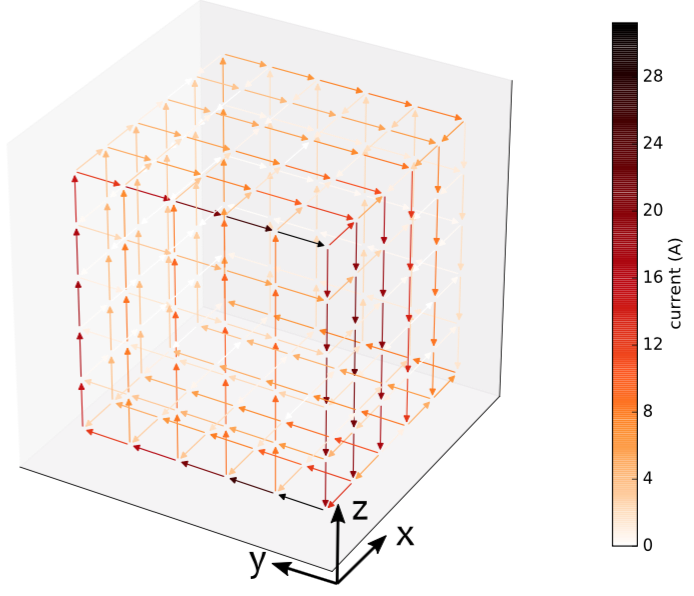
\includegraphics[width=.45\linewidth]{gfx/coil_dipole}}
%   \quad
%   \subfloat[XY section in the middle --- achieved relative compensation of the homogeneous field.]{
%     \label{fig:coils_dipole_section}
%     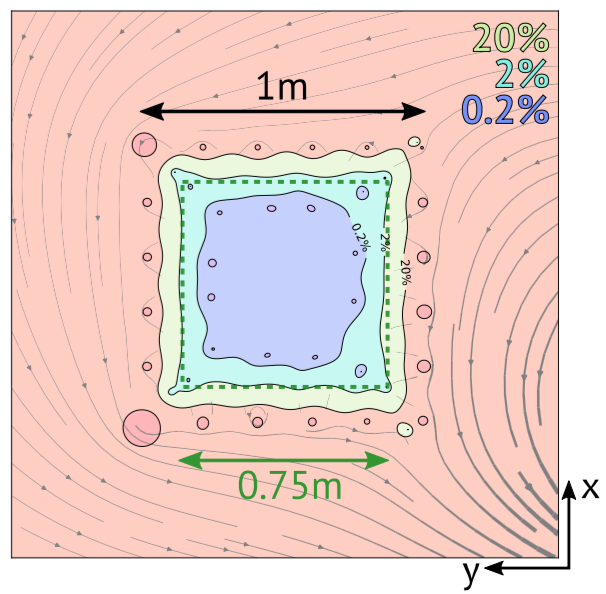
\includegraphics[width=.45\linewidth]{gfx/coil_dipole_section}}
%   \caption{Coils as a vector space.}
% \end{figure}



% \section{Construction}
% The first step is to define the \emph{coil surface}. Afterwards the surface has to be divided into tiles. The tiles need not necessarily be squared. They may not be rectangular, on even not flat. The finer the division, the better the field can be approximated, but also the harder it is to construct the system. A simple choice is to choose the coil surface to be a cuboid and the tiles to be rectangles.


% Exploit symmetries --- a homogeneous coil may be viewed a sum of a number of
% much simpler to construct coils, which are then connected in series.

% \begin{figure}
%   \centering
%   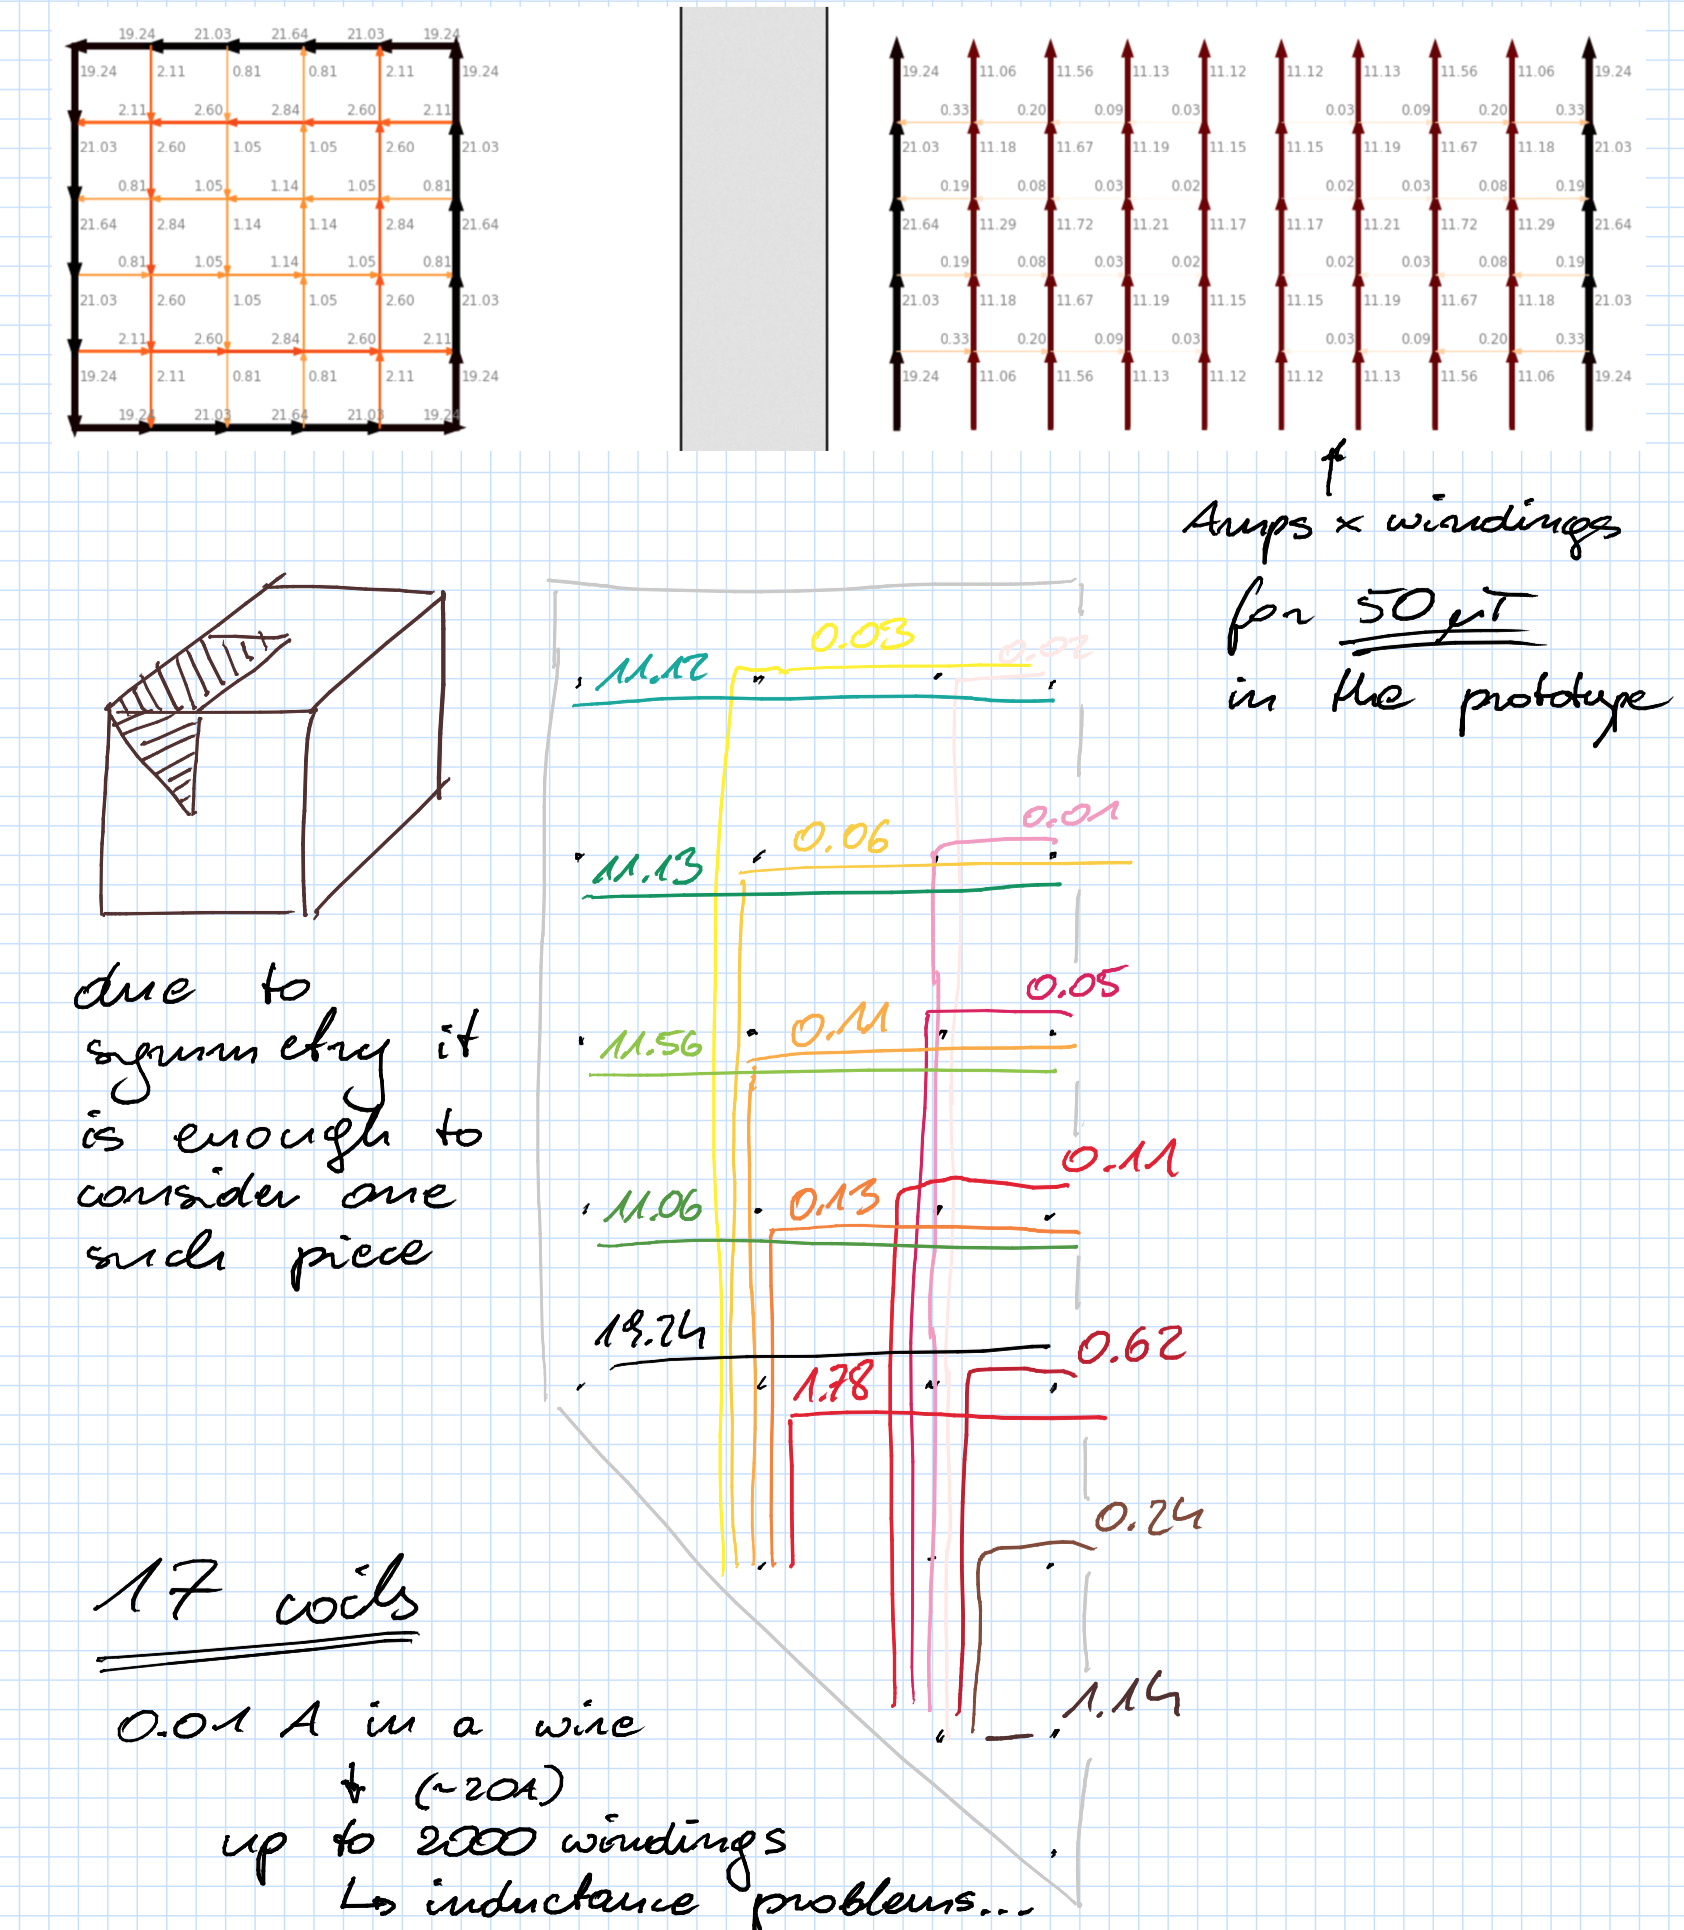
\includegraphics[width=.6\linewidth]{gfx/coils/wiring}
%   \caption
%   [TODO]
%   {%FIXME directly copied from the SFC paper
% The wiring solution.}
%   \label{fig:coils_wiring}
% \end{figure}

% Each edge can have any real current (albeit the Kirchoff law is fulfilled).
% However, to keep the number of control channels reasonably small, they need
% to be driven with one current source. Two techniques may be used:
% \begin{enumerate}
%   \item using a different number of wires, connected in series --- only discrete
%   \item varying resistance of different parts of the coil connected in parallel
%   --- can be adjusted continuously, but causes power dissipation.
% \end{enumerate}

% 1A, 0.1A, 0.001A wires solution --- keeps the number of windings reasonably small.
% With a simple use of additional resistors each coil may be still driven with only
% one power supply --- \emph{provide a figure}.

% \begin{figure}
%   \centering
%   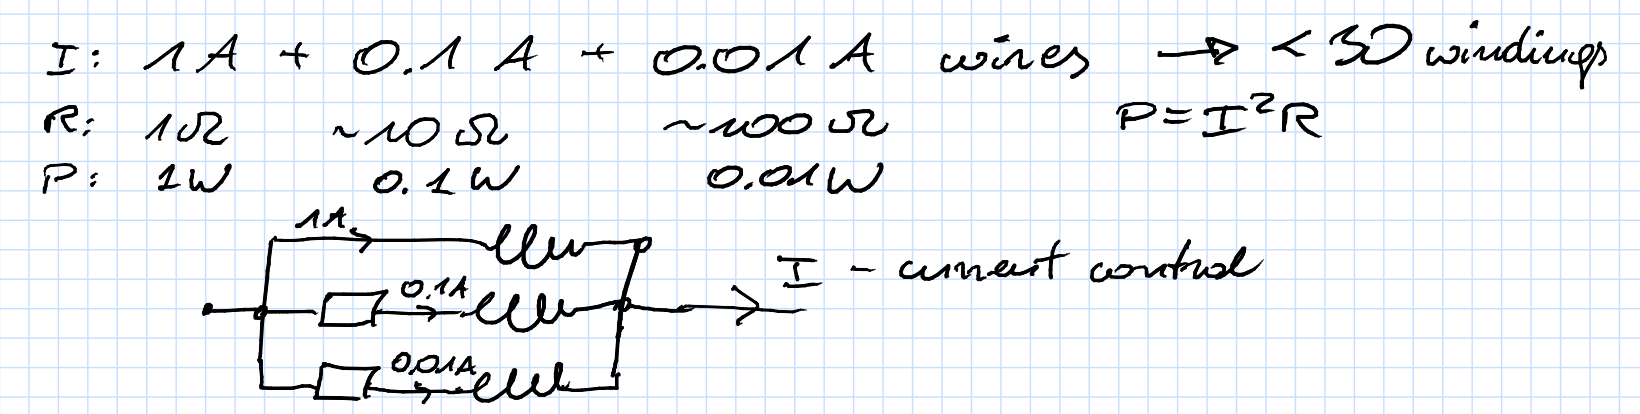
\includegraphics[width=.6\linewidth]{gfx/coils/current_discretisation}
%   \caption
%   [TODO]
%   {%FIXME directly copied from the SFC paper
% The wirining solution.}
%   \label{fig:coils_current_discretisation}
% \end{figure}

% Care has to be taken to balance voltage and current needs for the power supplies.

% Parameters to vary: number of windings, thickness of cable (price). Note also
% the inductance of the coils.

% \section{Possible generalisations}
% \begin{enumerate}
%   \item the surface does not need to be cubic
%   \item
% \end{enumerate}



% \section{Surrounding Field Compensation in the nEDM experiment}
% The main challenge of the nEDM experiment is reaching a magnetic field stability on the picotesla level on a timescale of minutes. At the same time the experiment is set up in a research facility, where strong magnets are common. In fact, at the experimental site the compass points in different directions throughout the day.

% The main part of attenuation of the magnetic field is done by four layers of \mbox{μ-metal} --- material with very high permeability (around 400\,000). However, \mbox{μ-metal}, being a ferromagnetic, is itself susceptible to become magnetised and and create a magnetic field of its own. In order to keep the magnetisation stable the \mbox{μ-metal} shield has been surrounded by a system of large coils. The coils are driven in a feedback loop with magnetic filed sensors (see Fig.\,\ref{fig:nEDM_SFC}). The system has been described in the paper \citep{Afach2014}.

% \begin{figure}
%   \centering
%   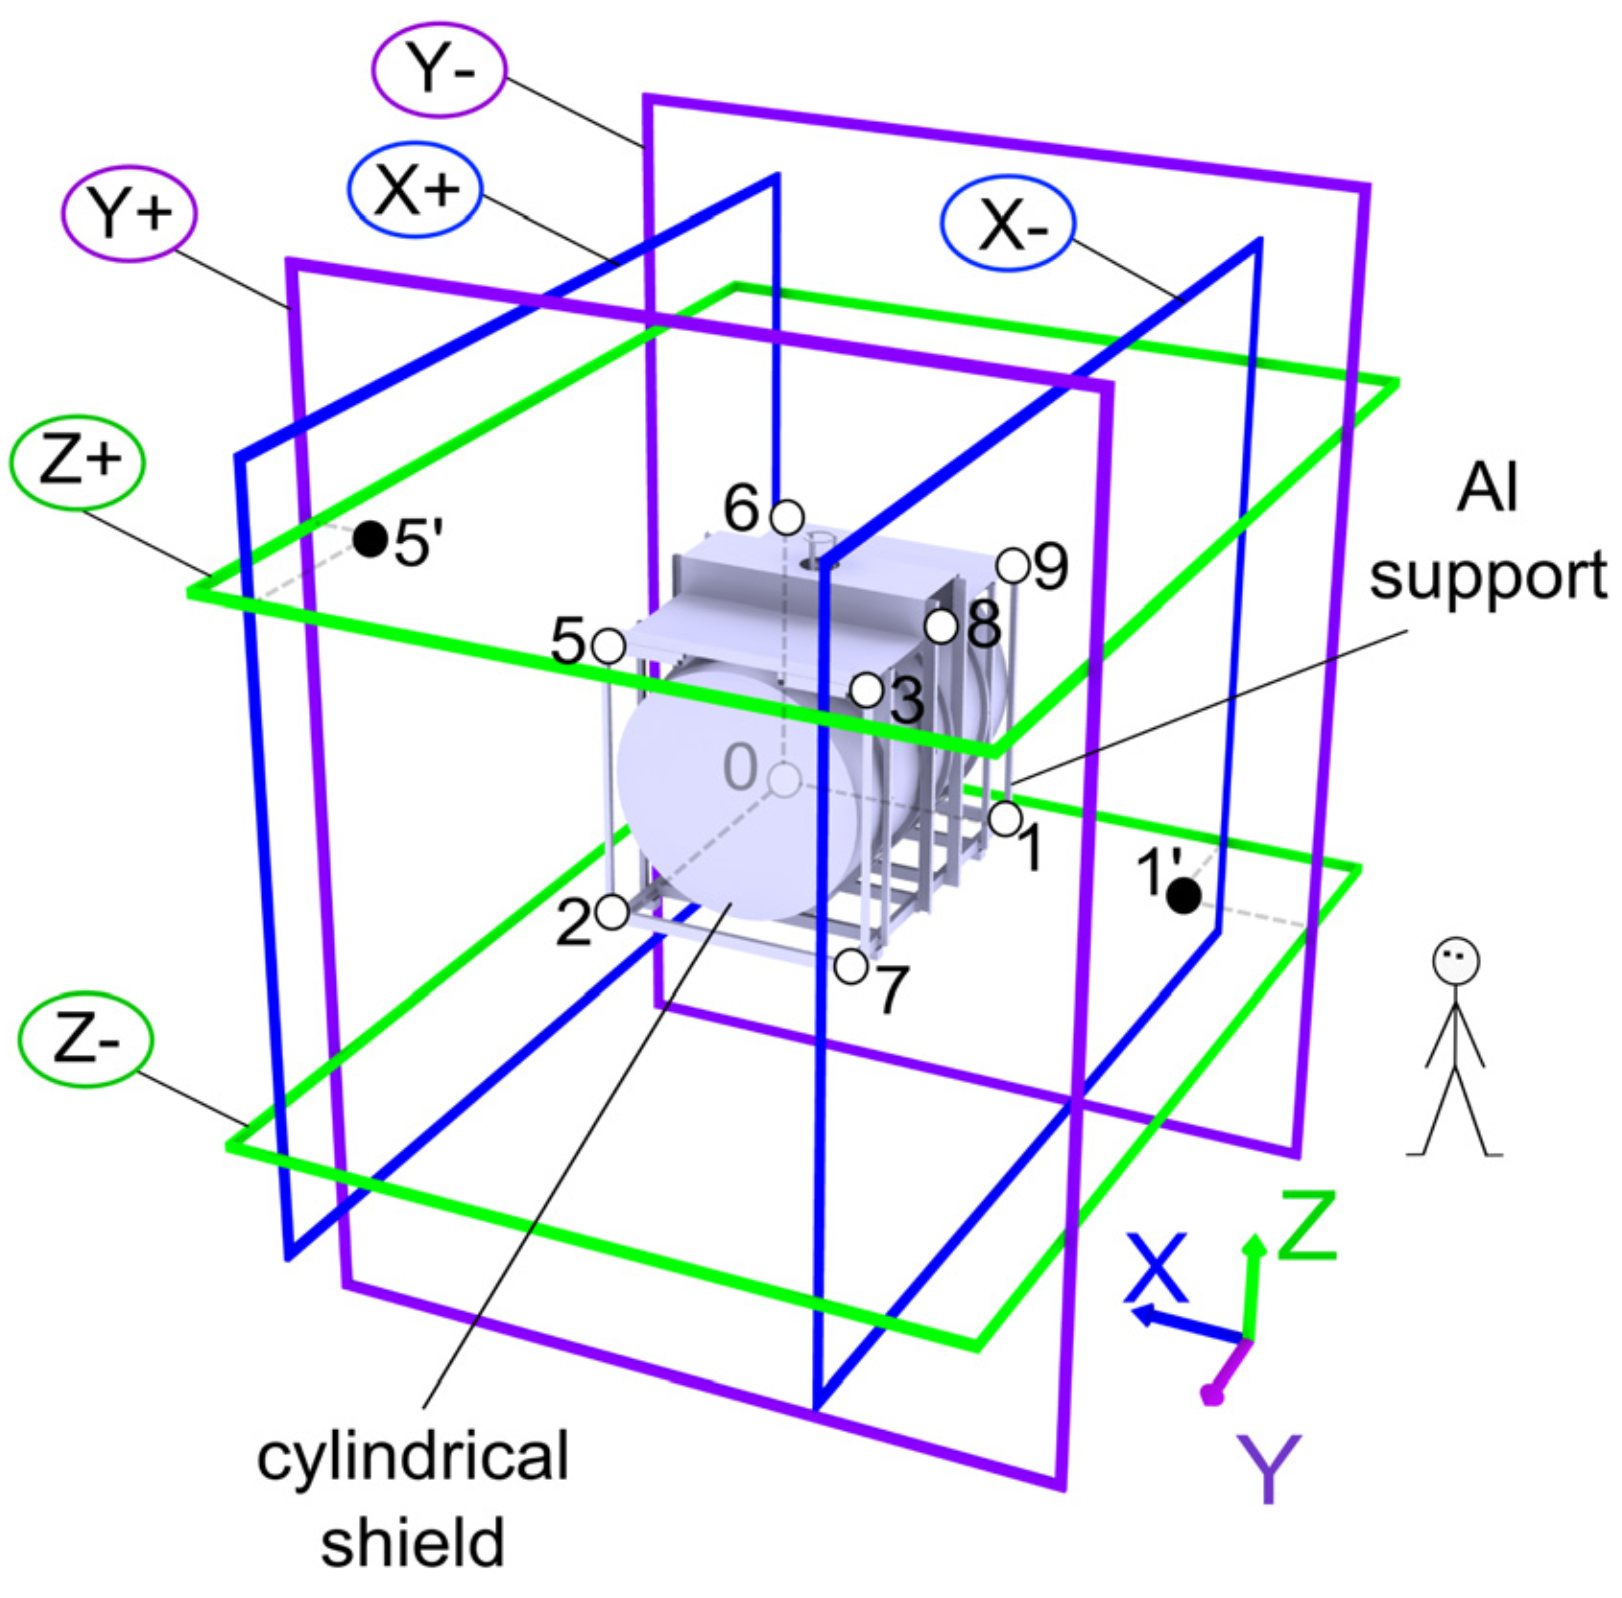
\includegraphics[width=.6\linewidth]{gfx/nEDM_SFC}
%   \caption
%   [Sketch of the nEDM SFC system.]
%   {%FIXME directly copied from the SFC paper
% Sketch of the SFC system consisting of six coils surrounding the Mu-metal magnetic shield of the nEDM spectrometer. The visible outermost layer of the cylindrical shield is mounted in its aluminum support structure.
% The Helmholtz coil pairs are labeled (X+, X-),(X-, Y-) and (Z+,Z-). The coordinate system of the experiment is given at the lower right. Its origin is at the center of the magnetic shield. Three--axis fluxgates (open circles) are mounted on the aluminium support of the experiment and numbered according to the fluxgate nomenclature given in the text. The positions 10 and 50 (full circles) depict previous locations of fluxgates FG 1 and FG 5 referred to in Sec. VB. FG 4 is omitted as it was removed from the system after a sensor failure.}
%   \label{fig:nEDM_SFC}
% \end{figure}

% The SFC system operates since 2013, attenuating the magnetic field by factor more than 5, even during ramping of nearby magnets.
